% ----------------------------------------------------------------------
%
%                            TFMTesis.tex
%
%----------------------------------------------------------------------
%
% Este fichero contiene el "documento maestro" del documento. Lo único
% que hace es configurar el entorno LaTeX e incluir los ficheros .tex
% que contienen cada sección.
%
%----------------------------------------------------------------------
%
% Los ficheros necesarios para este documento son:
%
%       TeXiS/* : ficheros de la plantilla TeXiS.
%       Cascaras/* : ficheros con las partes del documento que no
%          son capítulos ni apéndices (portada, agradecimientos, etc.)
%       Capitulos/*.tex : capítulos de la tesis
%       Apendices/*.tex: apéndices de la tesis
%       constantes.tex: constantes LaTeX
%       config.tex : configuración de la "compilación" del documento
%       guionado.tex : palabras con guiones
%
% Para la bibliografía, además, se necesitan:
%
%       *.bib : ficheros con la información de las referencias
%
% ---------------------------------------------------------------------

\documentclass[12pt,a4paper,twoside]{book}

%
% Definimos  el   comando  \compilaCapitulo,  que   luego  se  utiliza
% (opcionalmente) en config.tex. Quedaría  mejor si también se definiera
% en  ese fichero,  pero por  el modo  en el  que funciona  eso  no es
% posible. Puedes consultar la documentación de ese fichero para tener
% más  información. Definimos también  \compilaApendice, que  tiene el
% mismo  cometido, pero  que se  utiliza para  compilar  únicamente un
% apéndice.
%
%
% Si  queremos   compilar  solo   una  parte  del   documento  podemos
% especificar mediante  \includeonly{...} qué ficheros  son los únicos
% que queremos  que se incluyan.  Esto  es útil por  ejemplo para sólo
% compilar un capítulo.
%
% El problema es que todos aquellos  ficheros que NO estén en la lista
% NO   se  incluirán...  y   eso  también   afecta  a   ficheros  de
% la plantilla...
%
% Total,  que definimos  una constante  con los  ficheros  que siempre
% vamos a querer compilar  (aquellos relacionados con configuración) y
% luego definimos \compilaCapitulo.
\newcommand{\ficherosBasicosTeXiS}{%
TeXiS/TeXiS_pream,TeXiS/TeXiS_cab,TeXiS/TeXiS_bib,TeXiS/TeXiS_cover%
}
\newcommand{\ficherosBasicosTexto}{%
constantes,guionado,Cascaras/bibliografia,config%
}
\newcommand{\compilaCapitulo}[1]{%
\includeonly{\ficherosBasicosTeXiS,\ficherosBasicosTexto,Capitulos/#1}%
}

\newcommand{\compilaApendice}[1]{%
\includeonly{\ficherosBasicosTeXiS,\ficherosBasicosTexto,Apendices/#1}%
}

%- - - - - - - - - - - - - - - - - - - - - - - - - - - - - - - - - - -
%            Preámbulo del documento. Configuraciones varias
%- - - - - - - - - - - - - - - - - - - - - - - - - - - - - - - - - - -

% Define  el  tipo  de  compilación que  estamos  haciendo.   Contiene
% definiciones  de  constantes que  cambian  el  comportamiento de  la
% compilación. Debe incluirse antes del paquete TeXiS/TeXiS.sty
%---------------------------------------------------------------------
%
%                          config.tex
%
%---------------------------------------------------------------------
%
% Contiene la  definición de constantes  que determinan el modo  en el
% que se compilará el documento.
%
%---------------------------------------------------------------------
%
% En concreto, podemos  indicar si queremos "modo release",  en el que
% no  aparecerán  los  comentarios  (creados  mediante  \com{Texto}  o
% \comp{Texto}) ni los "por  hacer" (creados mediante \todo{Texto}), y
% sí aparecerán los índices. El modo "debug" (o mejor dicho en modo no
% "release" muestra los índices  (construirlos lleva tiempo y son poco
% útiles  salvo  para   la  versión  final),  pero  sí   el  resto  de
% anotaciones.
%
% Si se compila con LaTeX (no  con pdflatex) en modo Debug, también se
% muestran en una esquina de cada página las entradas (en el índice de
% palabras) que referencian  a dicha página (consulta TeXiS_pream.tex,
% en la parte referente a show).
%
% El soporte para  el índice de palabras en  TeXiS es embrionario, por
% lo  que no  asumas que  esto funcionará  correctamente.  Consulta la
% documentación al respecto en TeXiS_pream.tex.
%
%
% También  aquí configuramos  si queremos  o  no que  se incluyan  los
% acrónimos  en el  documento final  en la  versión release.  Para eso
% define (o no) la constante \acronimosEnRelease.
%
% Utilizando \compilaCapitulo{nombre}  podemos también especificar qué
% capítulo(s) queremos que se compilen. Si no se pone nada, se compila
% el documento  completo.  Si se pone, por  ejemplo, 01Introduccion se
% compilará únicamente el fichero Capitulos/01Introduccion.tex
%
% Para compilar varios  capítulos, se separan sus nombres  con comas y
% no se ponen espacios de separación.
%
% En realidad  la macro \compilaCapitulo  está definida en  el fichero
% principal tesis.tex.
%
%---------------------------------------------------------------------


% Comentar la línea si no se compila en modo release.
% TeXiS hará el resto.
% ¡¡¡Si cambias esto, haz un make clean antes de recompilar!!!
\def\release{1}


% Descomentar la linea si se quieren incluir los
% acrónimos en modo release (en modo debug
% no se incluirán nunca).
% ¡¡¡Si cambias esto, haz un make clean antes de recompilar!!!
%\def\acronimosEnRelease{1}


% Descomentar la línea para establecer el capítulo que queremos
% compilar

% \compilaCapitulo{01Introduccion}
% \compilaCapitulo{02EstructuraYGeneracion}
% \compilaCapitulo{03Edicion}
% \compilaCapitulo{04Imagenes}
% \compilaCapitulo{05Bibliografia}
% \compilaCapitulo{06Makefile}

% \compilaApendice{01AsiSeHizo}

% Variable local para emacs, para  que encuentre el fichero maestro de
% compilación y funcionen mejor algunas teclas rápidas de AucTeX
%%%
%%% Local Variables:
%%% mode: latex
%%% TeX-master: "./Tesis.tex"
%%% End:


% Paquete de la plantilla
\usepackage{TeXiS/TeXiS}

% Incluimos el fichero con comandos de constantes
%---------------------------------------------------------------------
%
%                          constantes.tex
%
%---------------------------------------------------------------------
%
% Fichero que  declara nuevos comandos LaTeX  sencillos realizados por
% comodidad en la escritura de determinadas palabras
%
%---------------------------------------------------------------------

%%%%%%%%%%%%%%%%%%%%%%%%%%%%%%%%%%%%%%%%%%%%%%%%%%%%%%%%%%%%%%%%%%%%%%
% Comando: 
%
%       \titulo
%
% Resultado: 
%
% Escribe el título del documento.
%%%%%%%%%%%%%%%%%%%%%%%%%%%%%%%%%%%%%%%%%%%%%%%%%%%%%%%%%%%%%%%%%%%%%%
\def\titulo{\textsc{TeXiS}: Una plantilla de \LaTeX\
  para Tesis y otros documentos}

%%%%%%%%%%%%%%%%%%%%%%%%%%%%%%%%%%%%%%%%%%%%%%%%%%%%%%%%%%%%%%%%%%%%%%
% Comando: 
%
%       \autor
%
% Resultado: 
%
% Escribe el autor del documento.
%%%%%%%%%%%%%%%%%%%%%%%%%%%%%%%%%%%%%%%%%%%%%%%%%%%%%%%%%%%%%%%%%%%%%%
\def\autor{Marco Antonio y Pedro Pablo G\'omez Mart\'in}

% Variable local para emacs, para  que encuentre el fichero maestro de
% compilación y funcionen mejor algunas teclas rápidas de AucTeX

%%%
%%% Local Variables:
%%% mode: latex
%%% TeX-master: "tesis.tex"
%%% End:


% Sacamos en el log de la compilación el copyright
%\typeout{Copyright Marco Antonio and Pedro Pablo Gomez Martin}

%
% "Metadatos" para el PDF
%
\ifpdf\hypersetup{%
    pdftitle = {\titulo},
    pdfsubject = {Plantilla de Tesis},
    pdfkeywords = {Plantilla, LaTeX, tesis, trabajo de
      investigación, trabajo de Master},
    pdfauthor = {\textcopyright\ \autor},
    pdfcreator = {\LaTeX\ con el paquete \flqq hyperref\frqq},
    pdfproducer = {pdfeTeX-0.\the\pdftexversion\pdftexrevision},
    }
    \pdfinfo{/CreationDate (\today)}
\fi


%- - - - - - - - - - - - - - - - - - - - - - - - - - - - - - - - - - -
%                        Documento
%- - - - - - - - - - - - - - - - - - - - - - - - - - - - - - - - - - -
\begin{document}

% Incluimos el  fichero de definición de guionado  de algunas palabras
% que LaTeX no ha dividido como debería
%----------------------------------------------------------------
%
%                          guionado.tex
%
%----------------------------------------------------------------
%
% Fichero con algunas divisiones de palabras que LaTeX no
% hace correctamente si no se le da alguna ayuda.
%
%----------------------------------------------------------------

\hyphenation{
% a
abs-trac-to
abs-trac-tos
abs-trac-ta
abs-trac-tas
ac-tua-do-res
a-gra-de-ci-mien-tos
ana-li-za-dor
an-te-rio-res
an-te-rior-men-te
apa-rien-cia
a-pro-pia-do
a-pro-pia-dos
a-pro-pia-da
a-pro-pia-das
a-pro-ve-cha-mien-to
a-que-llo
a-que-llos
a-que-lla
a-que-llas
a-sig-na-tu-ra
a-sig-na-tu-ras
a-so-cia-da
a-so-cia-das
a-so-cia-do
a-so-cia-dos
au-to-ma-ti-za-do
% b
batch
bi-blio-gra-fía
bi-blio-grá-fi-cas
bien
bo-rra-dor
boo-l-ean-expr
% c
ca-be-ce-ra
call-me-thod-ins-truc-tion
cas-te-lla-no
cir-cuns-tan-cia
cir-cuns-tan-cias
co-he-ren-te
co-he-ren-tes
co-he-ren-cia
co-li-bri
co-men-ta-rio
co-mer-cia-les
co-no-ci-mien-to
cons-cien-te
con-si-de-ra-ba
con-si-de-ra-mos
con-si-de-rar-se
cons-tan-te
cons-trucción
cons-tru-ye
cons-tru-ir-se
con-tro-le
co-rrec-ta-men-te
co-rres-pon-den
co-rres-pon-dien-te
co-rres-pon-dien-tes
co-ti-dia-na
co-ti-dia-no
crean
cris-ta-li-zan
cu-rri-cu-la
cu-rri-cu-lum
cu-rri-cu-lar
cu-rri-cu-la-res
% d
de-di-ca-do
de-di-ca-dos
de-di-ca-da
de-di-ca-das
de-rro-te-ro
de-rro-te-ros
de-sa-rro-llo
de-sa-rro-llos
de-sa-rro-lla-do
de-sa-rro-lla-dos
de-sa-rro-lla-da
de-sa-rro-lla-das
de-sa-rro-lla-dor
de-sa-rro-llar
des-cri-bi-re-mos
des-crip-ción
des-crip-cio-nes
des-cri-to
des-pués
de-ta-lla-do
de-ta-lla-dos
de-ta-lla-da
de-ta-lla-das
di-a-gra-ma
di-a-gra-mas
di-se-ños
dis-po-ner
dis-po-ni-bi-li-dad
do-cu-men-ta-da
do-cu-men-to
do-cu-men-tos
% e
edi-ta-do
e-du-ca-ti-vo
e-du-ca-ti-vos
e-du-ca-ti-va
e-du-ca-ti-vas
e-la-bo-ra-do
e-la-bo-ra-dos
e-la-bo-ra-da
e-la-bo-ra-das
es-co-llo
es-co-llos
es-tu-dia-do
es-tu-dia-dos
es-tu-dia-da
es-tu-dia-das
es-tu-dian-te
e-va-lua-cio-nes
e-va-lua-do-res
exis-ten-tes
exhaus-ti-va
ex-pe-rien-cia
ex-pe-rien-cias
% f
for-ma-li-za-do
% g
ge-ne-ra-ción
ge-ne-ra-dor
ge-ne-ra-do-res
ge-ne-ran
% h
he-rra-mien-ta
he-rra-mien-tas
% i
i-dio-ma
i-dio-mas
im-pres-cin-di-ble
im-pres-cin-di-bles
in-de-xa-do
in-de-xa-dos
in-de-xa-da
in-de-xa-das
in-di-vi-dual
in-fe-ren-cia
in-fe-ren-cias
in-for-ma-ti-ca
in-gre-dien-te
in-gre-dien-tes
in-me-dia-ta-men-te
ins-ta-la-do
ins-tan-cias
% j
% k
% l
len-gua-je
li-be-ra-to-rio
li-be-ra-to-rios
li-be-ra-to-ria
li-be-ra-to-rias
li-mi-ta-do
li-te-ra-rio
li-te-ra-rios
li-te-ra-ria
li-te-ra-rias
lo-tes
% m
ma-ne-ra
ma-nual
mas-que-ra-de
ma-yor
me-mo-ria
mi-nis-te-rio
mi-nis-te-rios
mo-de-lo
mo-de-los
mo-de-la-do
mo-du-la-ri-dad
mo-vi-mien-to
% n
na-tu-ral
ni-vel
nues-tro
% o
obs-tan-te
o-rien-ta-do
o-rien-ta-dos
o-rien-ta-da
o-rien-ta-das
% p
pa-ra-le-lo
pa-ra-le-la
par-ti-cu-lar
par-ti-cu-lar-men-te
pe-da-gó-gi-ca
pe-da-gó-gi-cas
pe-da-gó-gi-co
pe-da-gó-gi-cos
pe-rio-di-ci-dad
per-so-na-je
plan-te-a-mien-to
plan-te-a-mien-tos
po-si-ción
pre-fe-ren-cia
pre-fe-ren-cias
pres-cin-di-ble
pres-cin-di-bles
pri-me-ra
pro-ble-ma
pro-ble-mas
pró-xi-mo
pu-bli-ca-cio-nes
pu-bli-ca-do
% q
% r
rá-pi-da
rá-pi-do
ra-zo-na-mien-to
ra-zo-na-mien-tos
re-a-li-zan-do
re-fe-ren-cia
re-fe-ren-cias
re-fe-ren-cia-da
re-fe-ren-cian
re-le-van-tes
re-pre-sen-ta-do
re-pre-sen-ta-dos
re-pre-sen-ta-da
re-pre-sen-ta-das
re-pre-sen-tar-lo
re-qui-si-to
re-qui-si-tos
res-pon-der
res-pon-sa-ble
% s
se-pa-ra-do
si-guien-do
si-guien-te
si-guien-tes
si-guie-ron
si-mi-lar
si-mi-la-res
si-tua-ción
% t
tem-pe-ra-ments
te-ner
trans-fe-ren-cia
trans-fe-ren-cias
% u
u-sua-rio
Unreal-Ed
% v
va-lor
va-lo-res
va-rian-te
ver-da-de-ro
ver-da-de-ros
ver-da-de-ra
ver-da-de-ras
ver-da-de-ra-men-te
ve-ri-fi-ca
% w
% x
% y
% z
}
% Variable local para emacs, para que encuentre el fichero
% maestro de compilación
%%%
%%% Local Variables:
%%% mode: latex
%%% TeX-master: "./Tesis.tex"
%%% End:


% Marcamos  el inicio  del  documento para  la  numeración de  páginas
% (usando números romanos para esta primera fase).
\frontmatter
\pagestyle{empty}

%---------------------------------------------------------------------
%
%                          configCover.tex
%
%---------------------------------------------------------------------
%
% cover.tex
% Copyright 2009 Marco Antonio Gomez-Martin, Pedro Pablo Gomez-Martin
%
% This file belongs to the TeXiS manual, a LaTeX template for writting
% Thesis and other documents. The complete last TeXiS package can
% be obtained from http://gaia.fdi.ucm.es/projects/texis/
%
% Although the TeXiS template itself is distributed under the 
% conditions of the LaTeX Project Public License
% (http://www.latex-project.org/lppl.txt), the manual content
% uses the CC-BY-SA license that stays that you are free:
%
%    - to share & to copy, distribute and transmit the work
%    - to remix and to adapt the work
%
% under the following conditions:
%
%    - Attribution: you must attribute the work in the manner
%      specified by the author or licensor (but not in any way that
%      suggests that they endorse you or your use of the work).
%    - Share Alike: if you alter, transform, or build upon this
%      work, you may distribute the resulting work only under the
%      same, similar or a compatible license.
%
% The complete license is available in
% http://creativecommons.org/licenses/by-sa/3.0/legalcode
%
%---------------------------------------------------------------------
%
% Fichero que contiene la configuración de la portada y de la 
% primera hoja del documento.
%
%---------------------------------------------------------------------


% Pueden configurarse todos los elementos del contenido de la portada
% utilizando comandos.

%%%%%%%%%%%%%%%%%%%%%%%%%%%%%%%%%%%%%%%%%%%%%%%%%%%%%%%%%%%%%%%%%%%%%%
% Título del documento:
% \tituloPortada{titulo}
% Nota:
% Si no se define se utiliza el del \titulo. Este comando permite
% cambiar el título de forma que se especifiquen dónde se quieren
% los retornos de carro cuando se utilizan fuentes grandes.
%%%%%%%%%%%%%%%%%%%%%%%%%%%%%%%%%%%%%%%%%%%%%%%%%%%%%%%%%%%%%%%%%%%%%%
\tituloPortada{%
Diseño de un Controlador Horario Personalizado para Empleados
}


%%%%%%%%%%%%%%%%%%%%%%%%%%%%%%%%%%%%%%%%%%%%%%%%%%%%%%%%%%%%%%%%%%%%%%
% Título del documento en inglés:
% \tituloPortadaEng{titulo}
% Nota:
% Si no se define se utiliza el del \titulo. Este comando permite
% cambiar el título de forma que se especifiquen dónde se quieren
% los retornos de carro cuando se utilizan fuentes grandes.
%%%%%%%%%%%%%%%%%%%%%%%%%%%%%%%%%%%%%%%%%%%%%%%%%%%%%%%%%%%%%%%%%%%%%%
\tituloPortadaEng{%
Designing a Customized Employee Time Tracker
}

%%%%%%%%%%%%%%%%%%%%%%%%%%%%%%%%%%%%%%%%%%%%%%%%%%%%%%%%%%%%%%%%%%%%%%
% Autor del documento:
% \autorPortada{Nombre}
% Se utiliza en la portada y en el valor por defecto del
% primer subtítulo de la segunda portada.
%%%%%%%%%%%%%%%%%%%%%%%%%%%%%%%%%%%%%%%%%%%%%%%%%%%%%%%%%%%%%%%%%%%%%%
\autorPortada{Santiago Elias Rabbia}

%%%%%%%%%%%%%%%%%%%%%%%%%%%%%%%%%%%%%%%%%%%%%%%%%%%%%%%%%%%%%%%%%%%%%%
% Fecha de publicación:
% \fechaPublicacion{Fecha}
% Puede ser vacío. Aparece en la última línea de ambas portadas
%%%%%%%%%%%%%%%%%%%%%%%%%%%%%%%%%%%%%%%%%%%%%%%%%%%%%%%%%%%%%%%%%%%%%%
% Descomentar para que ponga siempre la fecha actual
%\fechaPublicacion{\today}
\fechaPublicacion{\textcolor{red}{Fecha publicación}}

%%%%%%%%%%%%%%%%%%%%%%%%%%%%%%%%%%%%%%%%%%%%%%%%%%%%%%%%%%%%%%%%%%%%%%
% Imagen de la portada (y escala)
% \imagenPortada{Fichero}
% \escalaImagenPortada{Numero}
% Si no se especifica, se utiliza la imagen TODO.pdf
%%%%%%%%%%%%%%%%%%%%%%%%%%%%%%%%%%%%%%%%%%%%%%%%%%%%%%%%%%%%%%%%%%%%%%
% imagen en blanco y negro
%\imagenPortada{Imagenes/Vectorial/escudoUCM}
%imagen en color
\imagenPortada{Imagenes/Bitmap/escudoUCMcolor}
\escalaImagenPortada{.2}

%%%%%%%%%%%%%%%%%%%%%%%%%%%%%%%%%%%%%%%%%%%%%%%%%%%%%%%%%%%%%%%%%%%%%%
% Tipo de documento.
% \tipoDocumento{Tipo}
% Para el texto justo debajo del escudo.
% Si no se indica, se utiliza "TESIS DOCTORAL".
%%%%%%%%%%%%%%%%%%%%%%%%%%%%%%%%%%%%%%%%%%%%%%%%%%%%%%%%%%%%%%%%%%%%%%
\tipoDocumento{Trabajo de Fin de Grado}

%%%%%%%%%%%%%%%%%%%%%%%%%%%%%%%%%%%%%%%%%%%%%%%%%%%%%%%%%%%%%%%%%%%%%%
% Institución/departamento asociado al documento.
% \institucion{Nombre}
% Puede tener varias líneas. Se utiliza en las dos portadas.
% Si no se indica aparecerá vacío.
%%%%%%%%%%%%%%%%%%%%%%%%%%%%%%%%%%%%%%%%%%%%%%%%%%%%%%%%%%%%%%%%%%%%%%
\institucion{%
Grado en Ingeniería Informática\\[0.2em]
Facultad de Informática\\[0.2em]
Universidad Complutense de Madrid
}

%%%%%%%%%%%%%%%%%%%%%%%%%%%%%%%%%%%%%%%%%%%%%%%%%%%%%%%%%%%%%%%%%%%%%%
% Director del trabajo.
% \directorPortada{Nombre}
% Se utiliza para el valor por defecto del segundo subtítulo, donde
% se indica quién es el director del trabajo.
% Si se fuerza un subtítulo distinto, no hace falta definirlo.
%%%%%%%%%%%%%%%%%%%%%%%%%%%%%%%%%%%%%%%%%%%%%%%%%%%%%%%%%%%%%%%%%%%%%%
\directorPortada{Gonzalo Méndez Pozo}


%%%%%%%%%%%%%%%%%%%%%%%%%%%%%%%%%%%%%%%%%%%%%%%%%%%%%%%%%%%%%%%%%%%%%%
% Colaborador en la dirección del trabajo.
% \colaboradorPortada{Nombre}
% Se utiliza para el valor por defecto del segundo subtítulo, donde
% se indica quién es el colaborador en la dirección del trabajo.
% Si se fuerza un subtítulo distinto, no hace falta definirlo.
%%%%%%%%%%%%%%%%%%%%%%%%%%%%%%%%%%%%%%%%%%%%%%%%%%%%%%%%%%%%%%%%%%%%%%
% \colaboradorPortada{\textcolor{red}{Colaborador 1\\Colaborador 2}}


%%%%%%%%%%%%%%%%%%%%%%%%%%%%%%%%%%%%%%%%%%%%%%%%%%%%%%%%%%%%%%%%%%%%%%
% Texto del primer subtítulo de la segunda portada.
% \textoPrimerSubtituloPortada{Texto}
% Para configurar el primer "texto libre" de la segunda portada.
% Si no se especifica se indica "Memoria que presenta para optar al
% título de Doctor en Informática" seguido del \autorPortada.
%%%%%%%%%%%%%%%%%%%%%%%%%%%%%%%%%%%%%%%%%%%%%%%%%%%%%%%%%%%%%%%%%%%%%%
\textoPrimerSubtituloPortada{%
\textbf{Trabajo de Fin de Grado en Ingeniería Informática}\\ [0.3em]
}

%%%%%%%%%%%%%%%%%%%%%%%%%%%%%%%%%%%%%%%%%%%%%%%%%%%%%%%%%%%%%%%%%%%%%%
% Texto del segundo subtítulo de la segunda portada.
% \textoSegundoSubtituloPortada{Texto}
% Para configurar el segundo "texto libre" de la segunda portada.
% Si no se especifica se indica "Dirigida por el Doctor" seguido
% del \directorPortada.
%%%%%%%%%%%%%%%%%%%%%%%%%%%%%%%%%%%%%%%%%%%%%%%%%%%%%%%%%%%%%%%%%%%%%%
\textoSegundoSubtituloPortada{%
\textbf{Convocatoria: }Junio \the\year%\\[0.2em]
%\textbf{Calificación: }\textit{\textcolor{red}{Nota}}
}

%%%%%%%%%%%%%%%%%%%%%%%%%%%%%%%%%%%%%%%%%%%%%%%%%%%%%%%%%%%%%%%%%%%%%%
% \explicacionDobleCara
% Si se utiliza, se aclara que el documento está preparado para la
% impresión a doble cara.
%%%%%%%%%%%%%%%%%%%%%%%%%%%%%%%%%%%%%%%%%%%%%%%%%%%%%%%%%%%%%%%%%%%%%%
%\explicacionDobleCara

%%%%%%%%%%%%%%%%%%%%%%%%%%%%%%%%%%%%%%%%%%%%%%%%%%%%%%%%%%%%%%%%%%%%%%
% \isbn
% Si se utiliza, aparecerá el ISBN detrás de la segunda portada.
%%%%%%%%%%%%%%%%%%%%%%%%%%%%%%%%%%%%%%%%%%%%%%%%%%%%%%%%%%%%%%%%%%%%%%
%\isbn{978-84-692-7109-4}


%%%%%%%%%%%%%%%%%%%%%%%%%%%%%%%%%%%%%%%%%%%%%%%%%%%%%%%%%%%%%%%%%%%%%%
% \copyrightInfo
% Si se utiliza, aparecerá información de los derechos de copyright
% detrás de la segunda portada.
%%%%%%%%%%%%%%%%%%%%%%%%%%%%%%%%%%%%%%%%%%%%%%%%%%%%%%%%%%%%%%%%%%%%%%
%\copyrightInfo{\autor}


%%
%% Creamos las portadas
%%
\makeCover

% Variable local para emacs, para que encuentre el fichero
% maestro de compilación
%%%
%%% Local Variables:
%%% mode: latex
%%% TeX-master: "../Tesis.tex"
%%% End:

%\include{Cascaras/autorizacion}
% +--------------------------------------------------------------------+
% | Dedication Page (Optional)
% +--------------------------------------------------------------------+

% \chapter*{Dedicatoria}

% \begin{flushright}
% \begin{minipage}[c]{8.5cm}
% \flushright{\textit{A Pedro Pablo y Marco Antonio, por crear TeXiS e iluminar nuestro camino}}
% \end{minipage}
% \end{flushright}
% +--------------------------------------------------------------------+
% | Acknowledgements Page (Optional)                                   |
% +--------------------------------------------------------------------+

% \chapter*{Agradecimientos}

% A Guillermo, por el tiempo empleado en hacer estas plantillas. A Adrián, Enrique y Nacho, por sus comentarios para mejorar lo que hicimos. Y a Narciso, a quien no le ha hecho falta el Anillo Único para coordinarnos a todos.












\chapter*{Resumen}

\section*{\tituloPortadaVal}

Cambios en las regulaciones modificaron el procedimiento por el cual los empleados fichan al entrar a sus trabajos en una compañía 
de gestión de instalaciones, volviendo obsoletos muchos dispositivos existentes. Se necesitaba una respuesta rápida, por lo que se 
desarrolló un dispositivo de fichaje rentable que utiliza microcontroladores, un PCB personalizado y una caja impresa en 3D.

Este dispositivo IoT debe ser responsivo, intuitivo de usar y ofrecer un servicio casi ininterrumpido, enviando información a través
de WiFi o datos celulares. El intercambio de datos se realiza por medio de API alojada en la nube, desarrollada usando Java Spring,
que pueden ser montada como un contenedor de Docker, o como una Google Cloud Function.

\section*{Palabras clave}
   
\noindent fichador, microcontrolador, pcb, impresión 3D, cloud API, IoT, programación asíncrona, Docker, GCP, Java Spring

   



\begin{otherlanguage}{english}
\chapter*{Abstract}

\section*{\tituloPortadaEngVal}

Regulatory changes have prompted a shift in employee clock-in procedures at Acciona Facility Services, rendering many existing 
devices obsolete. A swift response was necessary, leading to the development of a cost-effective clocking device utilizing 
microcontrollers, a custom PCB, and a 3D-printed case.

This IoT device has to be responsive, intuitive to use and offer close-to uninterruped service, sending information through WiFi 
or cellular data. Data exchange is facilitated through cloud-hosted APIs developed using Java Spring, hostable as Docker containers
or as Google Cloud Functions.

\section*{Keywords}

\noindent clocking device, microcontroller, pcb, 3D print, cloud API, IoT, asynchronous programming, Docker, GCP, Java Spring




% Si el trabajo se escribe en inglés, comentar esta línea y descomentar
% otra igual que hay justo antes de \end{document}
% \end{otherlanguage}

\ifx\generatoc\undefined
\else
%---------------------------------------------------------------------
%
%                          TeXiS_toc.tex
%
%---------------------------------------------------------------------
%
% TeXiS_toc.tex
% Copyright 2009 Marco Antonio Gomez-Martin, Pedro Pablo Gomez-Martin
%
% This file belongs to TeXiS, a LaTeX template for writting
% Thesis and other documents. The complete last TeXiS package can
% be obtained from http://gaia.fdi.ucm.es/projects/texis/
%
% This work may be distributed and/or modified under the
% conditions of the LaTeX Project Public License, either version 1.3
% of this license or (at your option) any later version.
% The latest version of this license is in
%   http://www.latex-project.org/lppl.txt
% and version 1.3 or later is part of all distributions of LaTeX
% version 2005/12/01 or later.
%
% This work has the LPPL maintenance status `maintained'.
% 
% The Current Maintainers of this work are Marco Antonio Gomez-Martin
% and Pedro Pablo Gomez-Martin
%
%---------------------------------------------------------------------
%
% Contiene  los  comandos  para  generar los  índices  del  documento,
% entendiendo por índices las tablas de contenidos.
%
% Genera  el  índice normal  ("tabla  de  contenidos"),  el índice  de
% figuras y el de tablas. También  crea "marcadores" en el caso de que
% se esté compilando con pdflatex para que aparezcan en el PDF.
%
%---------------------------------------------------------------------


% Primero un poquito de configuración...


% Pedimos que inserte todos los epígrafes hasta el nivel \subsection en
% la tabla de contenidos.
\setcounter{tocdepth}{2} 

% Le  pedimos  que nos  numere  todos  los  epígrafes hasta  el  nivel
% \subsubsection en el cuerpo del documento.
\setcounter{secnumdepth}{3} 


% Creamos los diferentes índices.

% Lo primero un  poco de trabajo en los marcadores  del PDF. No quiero
% que  salga una  entrada  por cada  índice  a nivel  0...  si no  que
% aparezca un marcador "Índices", que  tenga dentro los otros tipos de
% índices.  Total, que creamos el marcador "Índices".
% Antes de  la creación  de los índices,  se añaden los  marcadores de
% nivel 1.

\ifpdf
   \pdfbookmark{Índices}{indices}
\fi

% Tabla de contenidos.
%
% La  inclusión  de '\tableofcontents'  significa  que  en la  primera
% pasada  de  LaTeX  se  crea   un  fichero  con  extensión  .toc  con
% información sobre la tabla de contenidos (es conceptualmente similar
% al  .bbl de  BibTeX, creo).  En la  segunda ejecución  de  LaTeX ese
% documento se utiliza para  generar la verdadera página de contenidos
% usando la  información sobre los  capítulos y demás guardadas  en el
% .toc
\ifpdf
   \pdfbookmark[1]{Tabla de Contenidos}{tabla de contenidos}
\fi

\cabeceraEspecial{\'Indice}

\tableofcontents

\newpage 

% Índice de figuras
%
% La idea es semejante que para  el .toc del índice, pero ahora se usa
% extensión .lof (List Of Figures) con la información de las figuras.

\ifpdf
   \pdfbookmark[1]{Índice de figuras}{indice de figuras}
\fi

\cabeceraEspecial{\'Indice de figuras}

\listoffigures

\newpage

% Índice de tablas
% Como antes, pero ahora .lot (List Of Tables)

% \ifpdf
%    \pdfbookmark[1]{Índice de tablas}{indice de tablas}
% \fi

% \cabeceraEspecial{\'Indice de tablas}

% \listoftables

% \newpage

% Variable local para emacs, para  que encuentre el fichero maestro de
% compilación y funcionen mejor algunas teclas rápidas de AucTeX

%%%
%%% Local Variables:
%%% mode: latex
%%% TeX-master: "../Tesis.tex"
%%% End:

\fi

% Marcamos el  comienzo de  los capítulos (para  la numeración  de las
% páginas) y ponemos la cabecera normal
\mainmatter

\pagestyle{fancy}
\restauraCabecera


\chapter{Introduction and objectives}
\label{cap:introduction}
% \addcontentsline{toc}{chapter}{Introduction}


Recent legislative changes introduced by both the Spanish Data Protection Agency and the national government 
have mandated alterations to employee clocking procedures. Notably, Spain now requires employees to clock in 
upon arrival at work, necessitating the implementation of reliable time-tracking systems 
\cite{boe_obligacionfichajes}. Additionally, the Spanish Data Protection Agency has banned the use of clocking 
devices employing biometric identification methods such as fingerprint scanning or facial recognition 
\cite{aepd_prohibicionbiometricos}.

A particular company manages many thousands of employees throughout Spain, and it was of utmost importance
to expeditely replace the non-compliant devices for different ones, as many companies were already being
imposed hefty fines, from tens to hundreds of thousands of Euros, for not meeting the new regulatory 
requirements.

The company already had providers for many types of clocking devices, and many of them were compliant, but 
were priced in the hundreds of Euros each. Now, faced with having to replace them, the prospect of replacing 
\textit{thousands} of units at considerable expense loomed large.  Moreover, outsourcing these devices often 
meant committing to complex time-tracking ecosystems, adding further complications and increasing the
complexity of the data the company manages.

These issues were brought to light to the innovation team at the company, and were then tasked with bringing 
a solution to market.

\section{Objectives}

Given the preceding challenges and considerations, the development of a cost-effective device and the establishment 
of a cloud infrastructure were deemed necessary.

The objectives of this project are as follows:
\begin{itemize}
    \item \textbf{Design and Prototyping}: Design a device utilizing microcontrollers and additional electronic 
    modules, such as LCD displays and NFC readers, to fulfill the specified requirements.
    \item \textbf{PCB Design}: Develop a Printed Circuit Board (PCB) layout to facilitate easy interconnection of 
    the various electronic modules used in the device, ensuring efficient and reliable performance.
    \item \textbf{API Development}: Create an Application Programming Interface (API) capable of deployment as a 
    Docker container or Google Cloud Function, enabling seamless communication between the device and cloud-based services.
    \item \textbf{Microcontroller Research}: Investigate the constraints and capabilities of microcontrollers, particularly 
    RP2040-based microcontrollers, to inform design decisions and optimize performance.
    \item \textbf{3D Printing and Modeling}: Explore the fundamentals of 3D printing and 3D modeling necessary for 
    designing a suitable enclosure for the device. Additionally, provide an overview and comparison of various materials 
    suitable for enclosure fabrication, considering factors such as durability, cost, and aesthetic appeal.
    \item \textbf{Cost Analysis}: Conduct a brief cost comparison between the new solution and the previous system, 
    demonstrating the financial benefits of the new design.
\end{itemize}

\chapter{Breadboard Prototype}
\label{cap:breadboardPrototype}

The first phase of developing the new clocking device involved thorough research into available components and 
microcontrollers in the market. Factors such as cost, functionality, and potential drawbacks were carefully 
evaluated to inform the selection process. Subsequently, selected components were tested by constructing a 
basic prototype on a breadboard to assess functionality and performance. Demonstrating the viability of the 
project at this stage was crucial for ensuring its continued development and success.

\section{Hardware selection}

Firstly, considering that the development was urgent, it would only be possible to use an already made 
controller. There were two routes to take:
\begin{itemize}
	\item Using a \textbf{single-board computer}.
	\item Using a \textbf{microcontroller}.
\end{itemize}

The team's familiarity with \textit{Raspberry Pi} products and their reputation for reliability led to the 
decision to utilize their offerings for the project. Given the lightweight processing requirements, the 
\textit{Raspberry Pi Zero W}, a cost-effective single-board computer with built-in WiFi capabilities, emerged 
as a suitable option. Alternatively, the \textit{Raspberry Pi Pico W}, a microcontroller, presented another 
viable choice.

However, it's important to note that while the \textit{Pi Zero} offers more features and functionality, it 
comes at a higher cost compared to the \textit{Pi Pico}. In fact, it costs almost three times as much. 
Therefore, careful consideration is warranted to determine whether the additional expense justifies the benefits.

%
% Single-board Computers
%
\subsection{Single-board Computers}

A single-board computer (\textit{SBC}) is a complete computer built on a single circuit board. It integrates all 
the necessary components required for a functional computer system, including a central processing unit (CPU), 
memory (RAM), storage (usually in the form of a MicroSD card), input/output ports, and sometimes additional 
features such as networking capabilities (e.g., Ethernet or WiFi), audio/video output, GPIO (General Purpose 
Input/Output) pins for connecting external devices, and even USB ports.

SBCs are designed to be compact and efficient, which is the case of the \textit{Pi Zero}, measuring about 65mm by 
30mm while drawing about one Watt of power. Additionally, SBCs can run an operating system, such as Ubuntu.

This ability to run an entire operating system significantly enhances their versatility compared to microcontrollers 
out-of-the-box. Many peripheral devices can simply be plugged into a USB port and function seamlessly without 
requiring additional configuration. For instance, a 3G SIM card adapter, which will be necessary for future stages 
of the project, can be effortlessly integrated into the system, letting the operating system take charge of the 
communication with the mobile network, abstracting all these problems from the programmer.


%
% Microcontrollers
%
\subsection{Microcontrollers}

A microcontroller is a compact integrated circuit (IC) that contains a central processing unit (CPU), memory (both 
volatile RAM and non-volatile flash memory), input/output peripherals (such as digital and analog I/O pins), and 
various other hardware components necessary for interfacing with external devices. Unlike single-board computers, 
microcontrollers are typically designed for specific tasks and embedded applications, often with real-time requirements.

One key characteristic of microcontrollers is their ability to execute dedicated firmware or software code stored in 
their internal memory. This code typically controls the behavior of the microcontroller, processes inputs from sensors 
or other external devices, and generates outputs to control actuators or display information.

The \textit{Raspberry Pi Pico W} is a development board that utilizes the \textit{RP2040} microcontroller chip. This board 
offers a range of features beyond its microcontroller, including onboard flash memory for program storage, versatile 
GPIO pins for interfacing with external devices, built-in USB connectivity for programming and power supply, and 
WiFi connectivity.

In comparison to single-board computers, the \textit{Pi Pico} does not have an operating system. Instead, firmware can be 
loaded onto it, and it is this firmware that provides functionality to the board. This firmware allows the programmer to 
use programming languages such as C or MicroPython, which then control the microcontroller's behavior and interactions with 
external devices.

The absence of an operating system reduces the overhead associated with system management and resource allocation, resulting 
in faster boot times and improved reliability for time-critical tasks.

Taking into account our previously established requirements, which prioritize minimal points of failure, low computational 
demands, and cost-effectiveness, the logical preference leans towards the utilization of a microcontroller. For instance, 
single-board computers often rely on SD cards for storage, which can be prone to failure after prolonged use due to factors 
such as wear and tear or data corruption. In contrast, microcontrollers typically have simpler storage mechanisms, such as 
onboard flash memory, which are less susceptible to such issues. Thus, lower operating costs.

As a conclusion, a \textbf{microcontroller will be used}, and in particular, the \textit{\textbf{Raspberry Pi Pico W}}.

\subsection{Electronic Modules}


% \begin{figure}[h]
% 	\centering
% 	
\includegraphics[width = 0.5\textwidth]{Imagenes/Vectorial/Todo.pdf}
% 	\caption{Ejemplo de imagen}
% 	\label{fig:sampleImage}
% \end{figure}

% Si te sirve de utilidad,  puedes incluir tablas para mostrar resultados, tal como se ve en la tabla \ref{tab:sampleTable}.


% \begin{table}
% 	\centering
% 	\begin{tabular}{c|c|c}
% 		\textbf{Col 1} & \textbf{Col 2} & \textbf{Col 3} \\
% 		\hline\hline
% 		3 & 3.01 & 3.50\\
% 		6 & 2.12 & 4.40\\
% 		1 & 3.79 & 5.00\\
% 		2 & 4.88 & 5.30\\
% 		4 & 3.50 & 2.90\\
% 		5 & 7.40 & 4.70\\
% 		\hline
% 	\end{tabular}
% 	\caption{Tabla de ejemplo}
% 	\label{tab:sampleTable}
% \end{table}

\chapter{PCB Design}
\label{cap:pcbdesign}

Following the initial development on a breadboard, the natural progression in the design evolution was to 
transition to a perfboard assembly. This intermediate step not only served to condense the device's 
footprint but also offered a preliminary glimpse into its form and functionality. Subsequently, the 
culmination of this iterative process involved the design and fabrication of a PCB tailored to the 
project's specifications, marking a significant milestone in its realization.


\section{Assembling on a Perfboard}

Perfboards, short for perforated boards, are commonly used prototyping platforms in electronics. They 
consist of a board with a grid of holes spaced at regular intervals. These holes are surrounded by copper 
pads or traces that can be connected using solder to create electronic circuits. Perfboards allow 
electronic components, such as resistors, capacitors, integrated circuits, and other discrete components, 
to be soldered onto the board, facilitating the creation of temporary or semi-permanent circuits for 
testing and development purposes \cite{perfboard}. They serve as a practical and versatile tool for 
electronics hobbyists, engineers, and designers to quickly prototype and iterate on circuit designs 
before moving to more permanent solutions like printed circuit boards (PCBs). Examples can be seen in 
Figures \ref{fig:perfboard_back} and \ref{fig:perfboard_front}.

\begin{figure}[h]
    \centering
    \begin{minipage}[b]{0.45\textwidth}
        \centering
        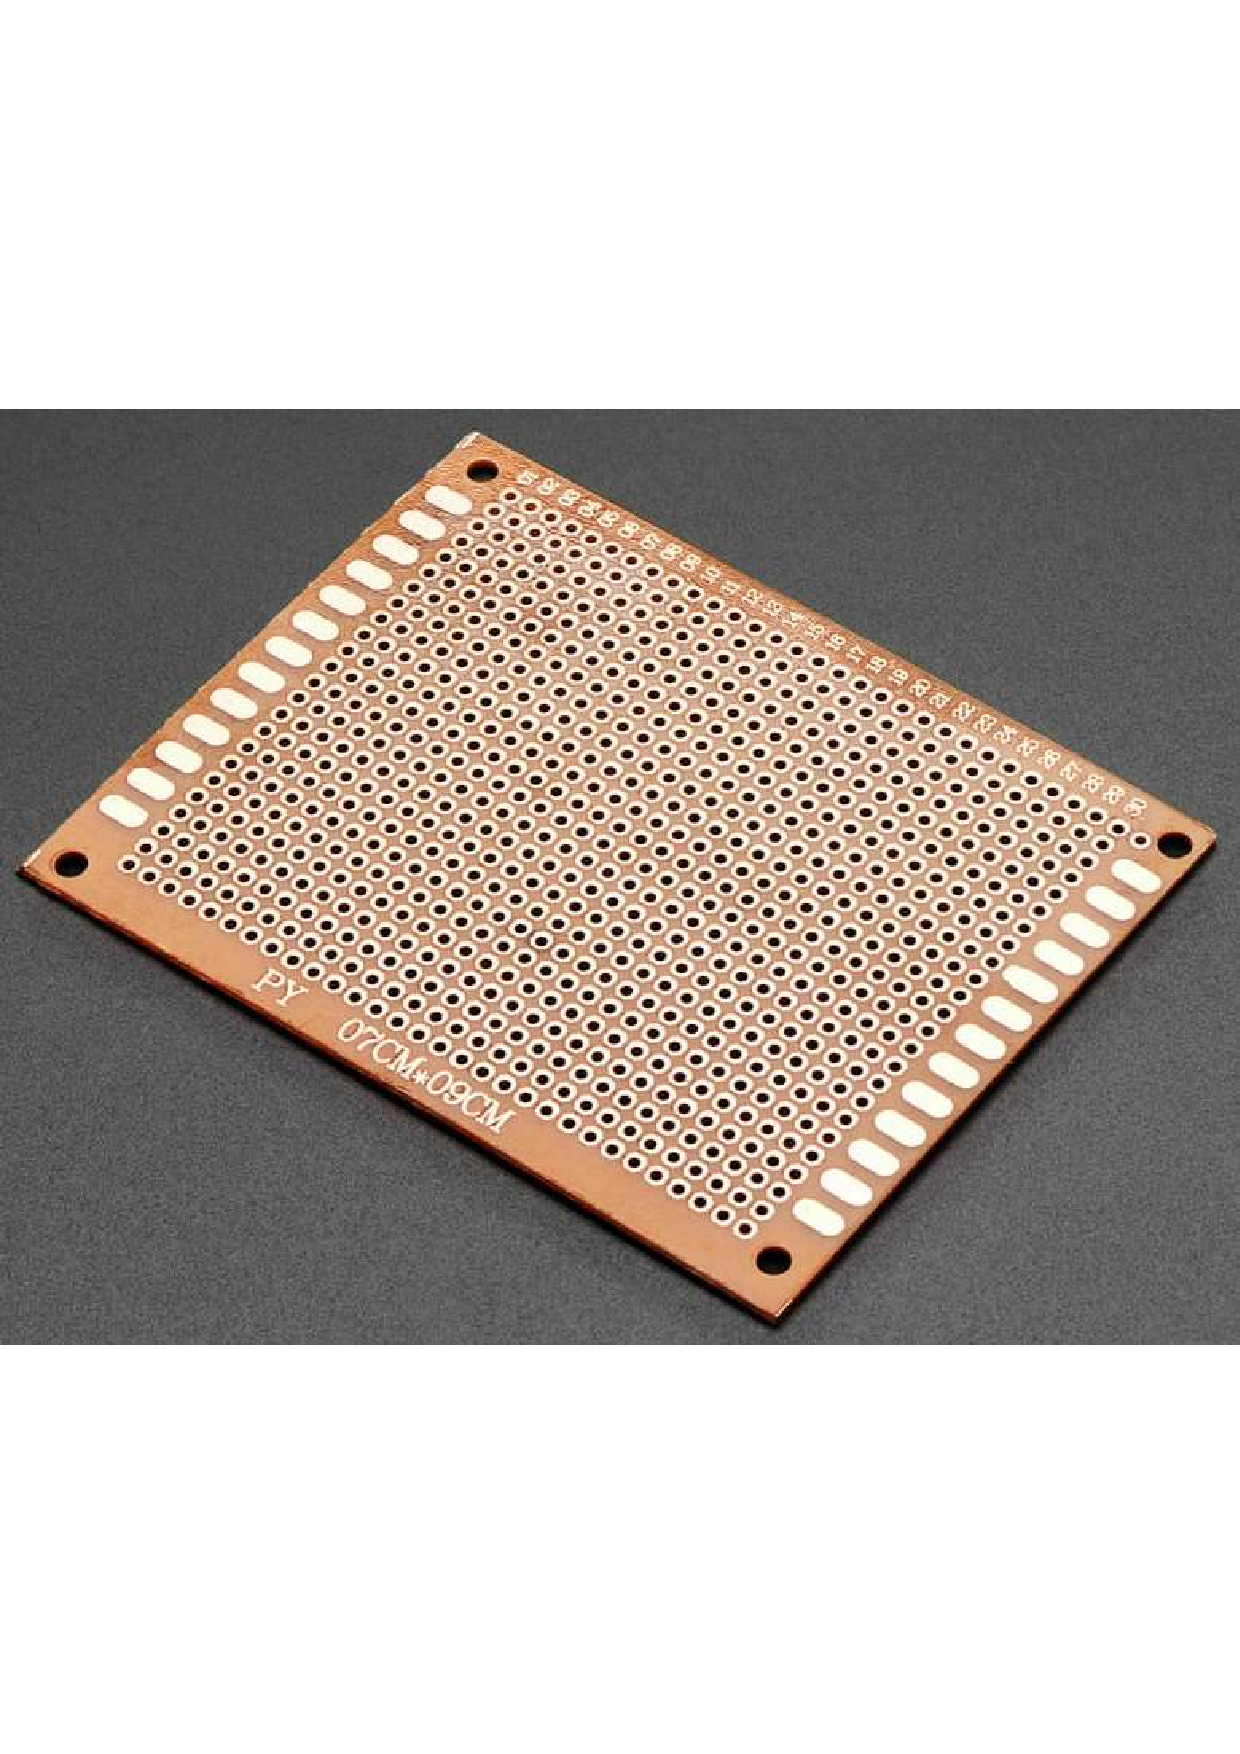
\includegraphics[width=.8\textwidth]{Imagenes/Vectorial/perfboard_back.pdf}
        \caption{Back side of a perfboard}
        \label{fig:perfboard_back}
    \end{minipage}
    \hfill
    \begin{minipage}[b]{0.45\textwidth}
        \centering
        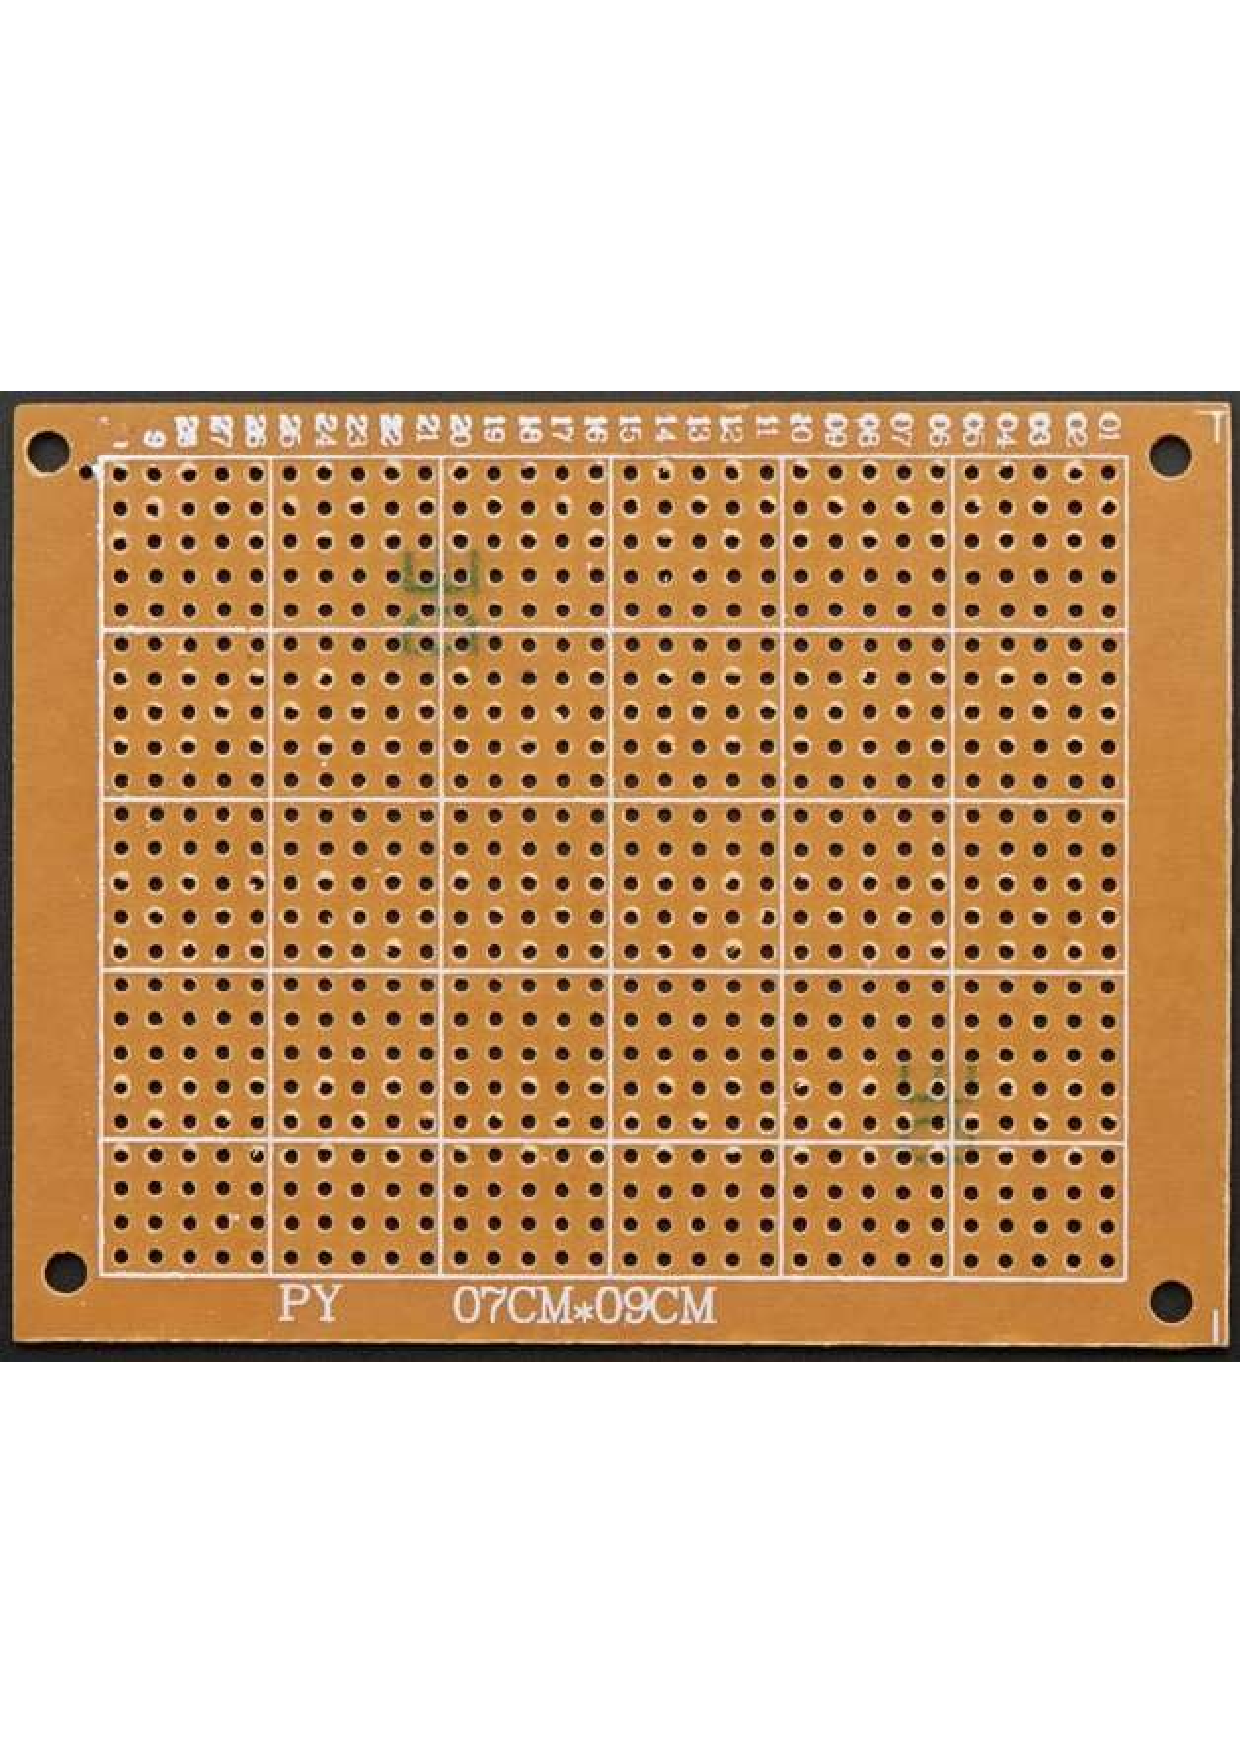
\includegraphics[width=.8\textwidth]{Imagenes/Vectorial/perfboard_front.pdf}
        \caption{Front side of a perfboard}
        \label{fig:perfboard_front}
    \end{minipage}
\end{figure}

In the context of this project, transitioning to a perfboard prototype served multiple crucial purposes. 
Firstly, it offered a tangible visualization of the future device's physical footprint, providing 
executives with a concrete representation of the project's direction and potential. This visual aid not 
only conveyed the scale and form of the device but also showed its feasibility and progress, instilling 
confidence in its development trajectory.

To commence this phase, a diagram detailing the placement of each component and its connection to the 
corresponding pins on the microcontroller was drafted. This diagram served as a blueprint, guiding the 
subsequent assembly process.

With the schematic as a roadmap, the assembly of the perfboard prototype commenced. Components were 
transitioned from the breadboard to the perfboard, ensuring each element found its designated place. 
Careful consideration was given to the layout, optimizing spatial organization for efficient circuitry 
and minimal interference.

\begin{figure}[h]
    \centering
    \begin{minipage}[b]{0.45\textwidth}
        \centering
        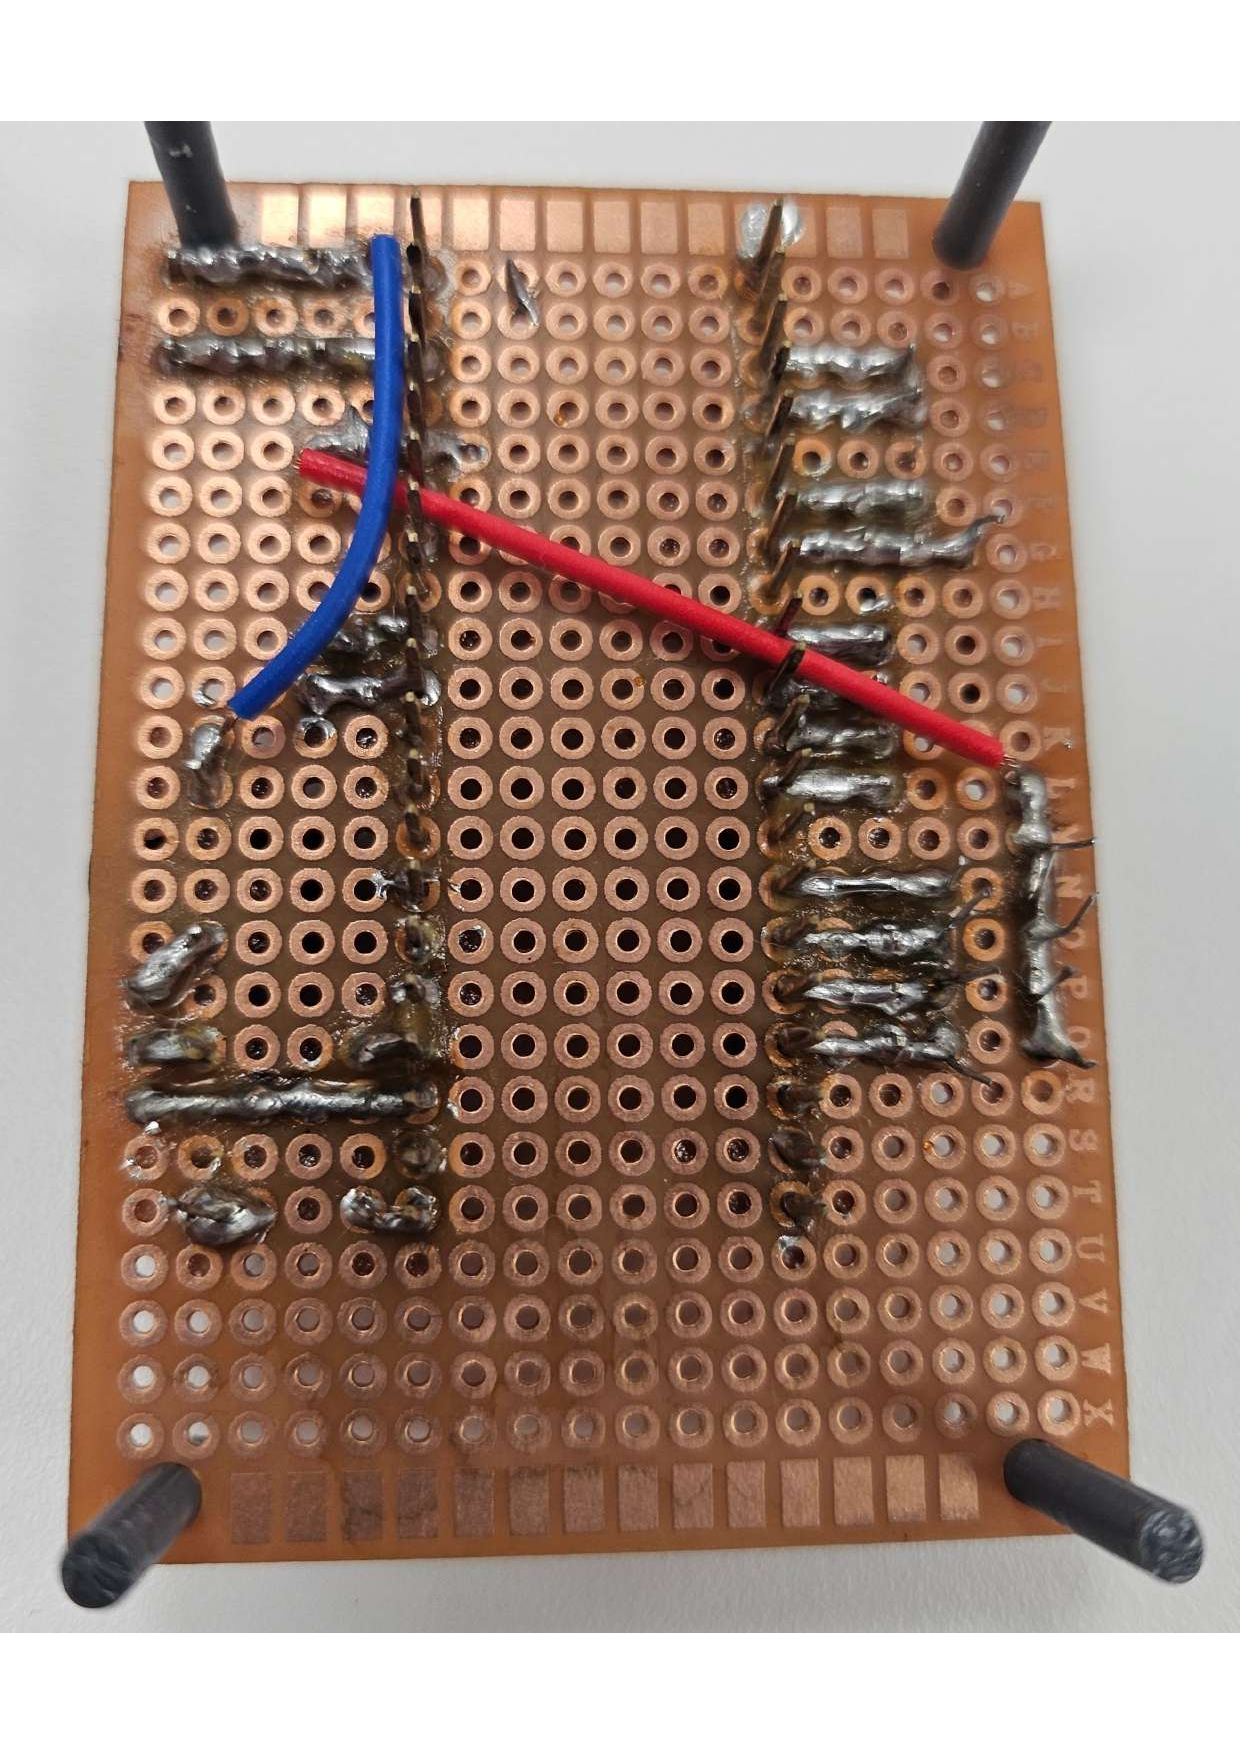
\includegraphics[width=.8\textwidth]{Imagenes/Vectorial/perfboard_assembled_back.pdf}
        \caption{Back side of the assembled perfboard}
        \label{fig:perfboard_assembled_back}
    \end{minipage}
    \hfill
    \begin{minipage}[b]{0.45\textwidth}
        \centering
        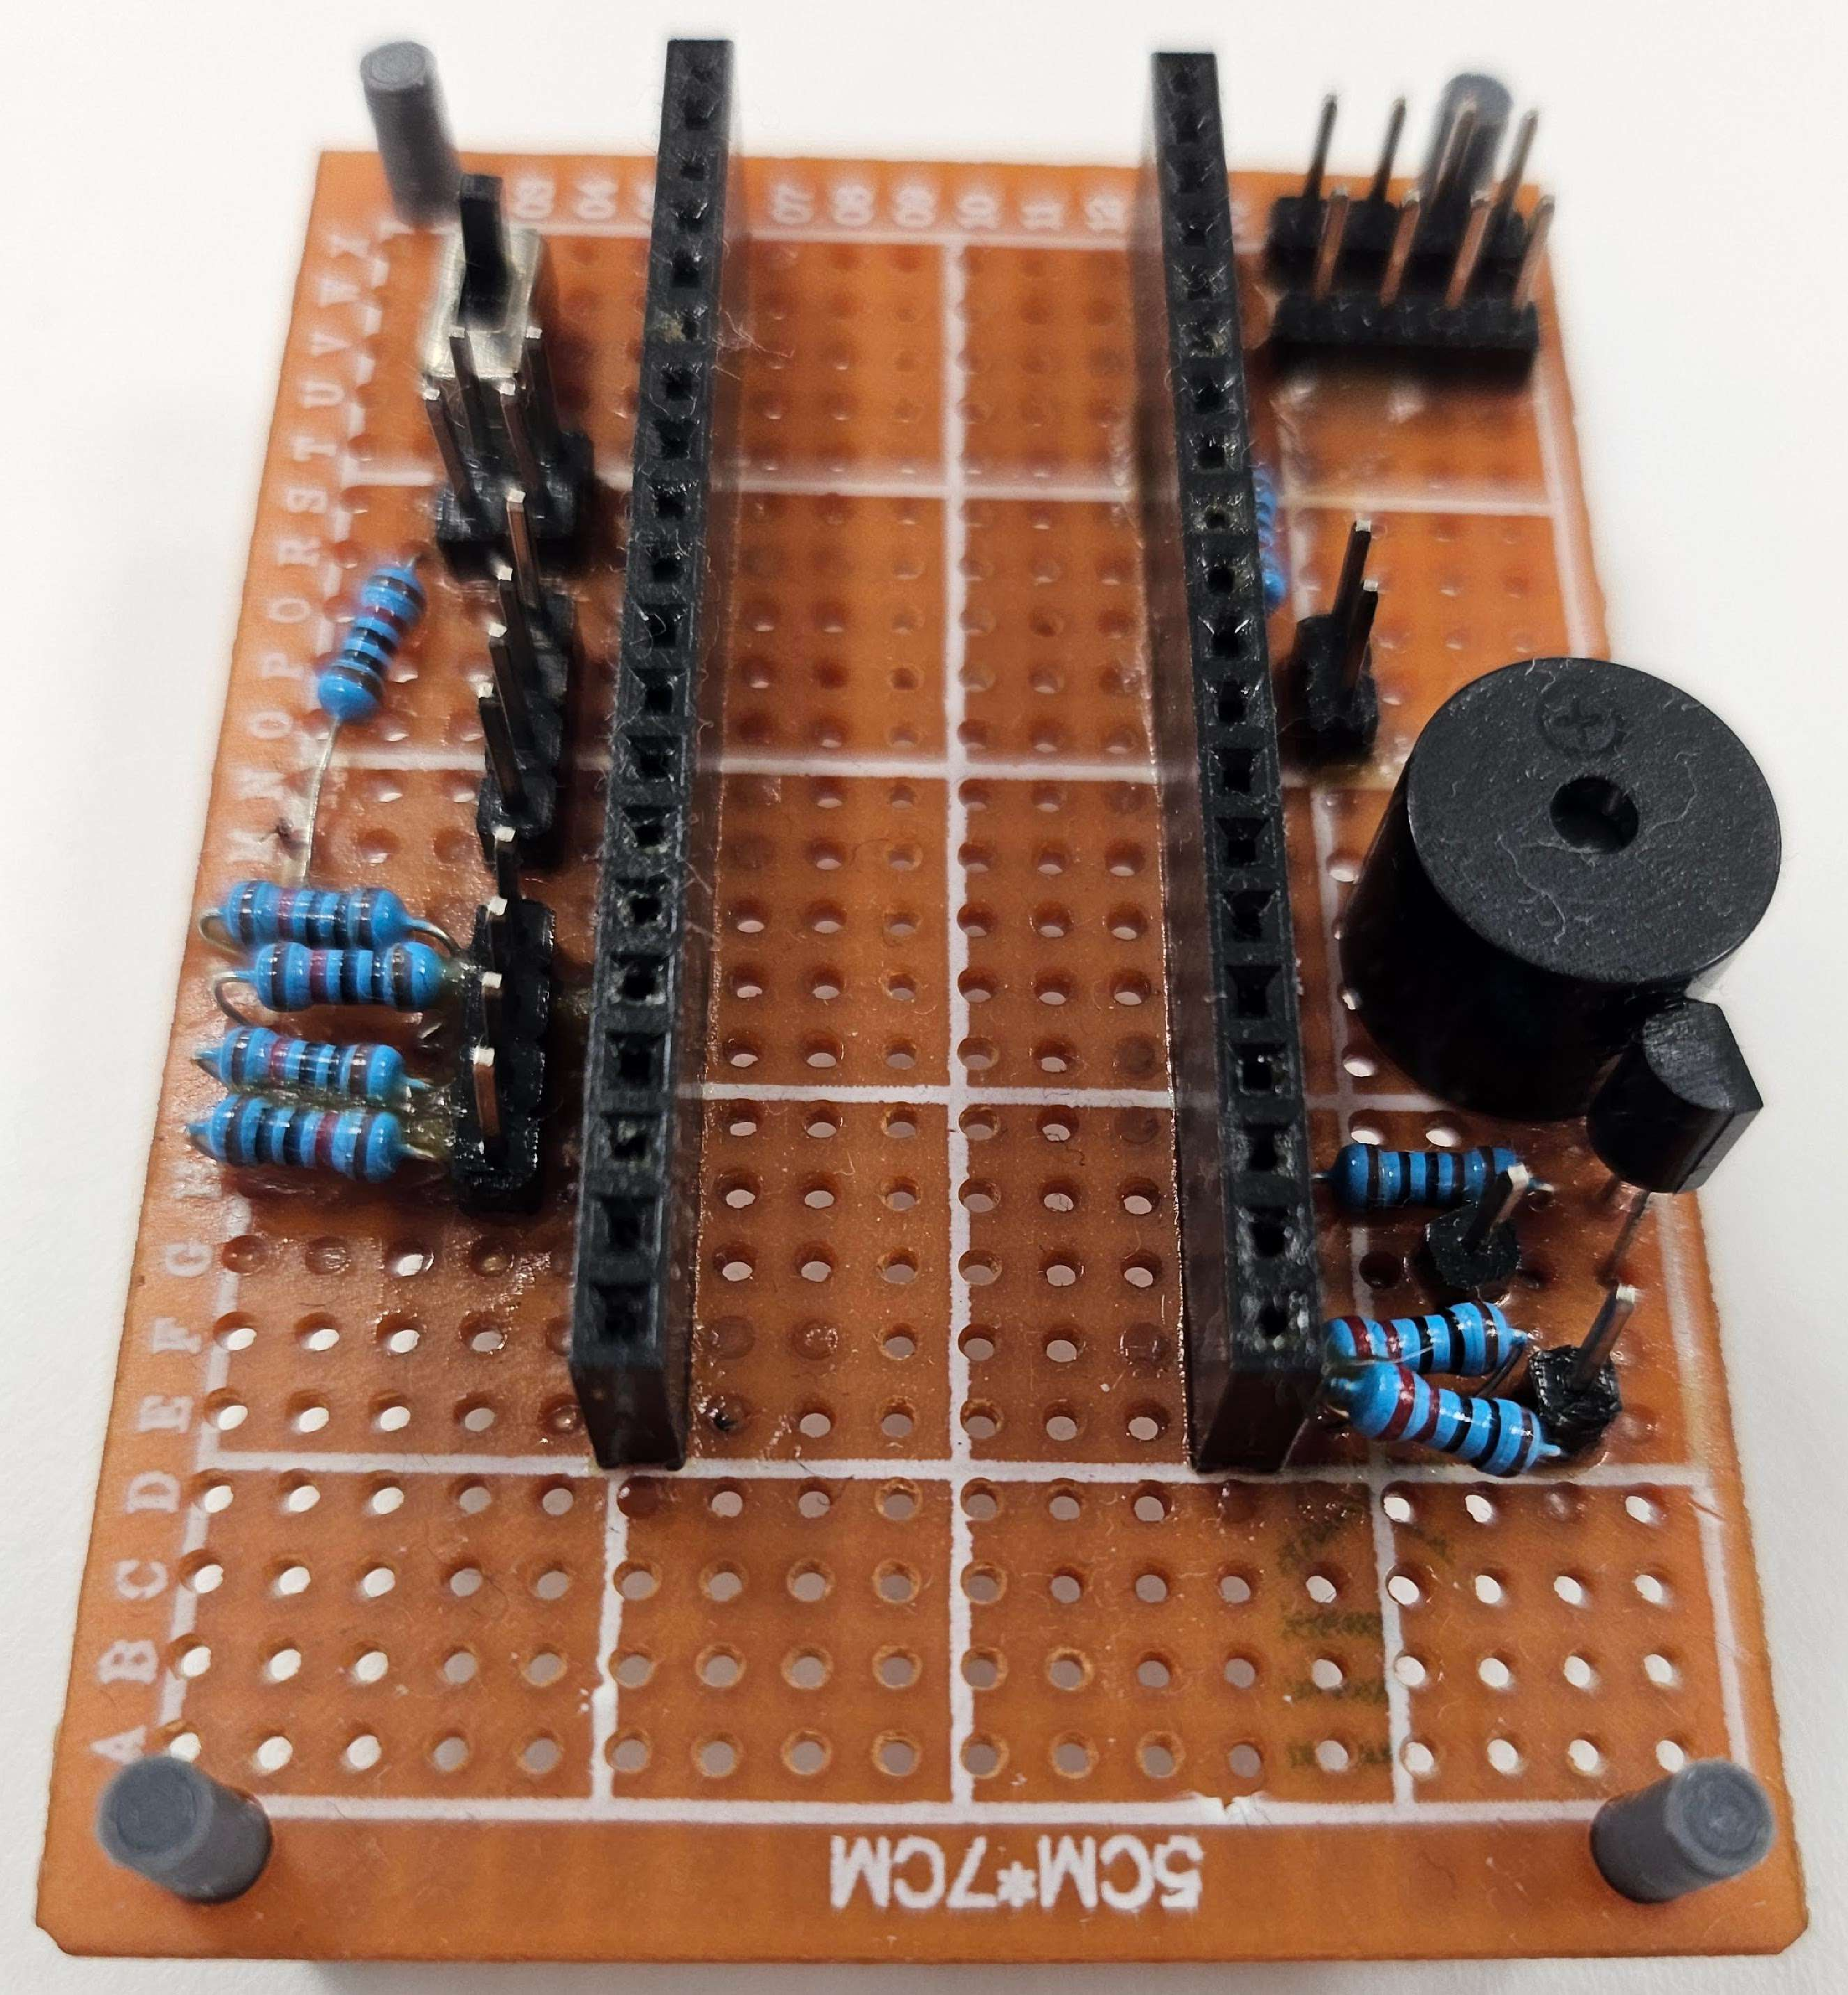
\includegraphics[width=.8\textwidth]{Imagenes/Vectorial/perfboard_assembled_front.pdf}
        \caption{Front side of the assembled perfboard}
        \label{fig:perfboard_assembled_front}
    \end{minipage}
\end{figure}


\section{Designing the PCB}

Now that the perfboard provided a good idea of how the PCB could be, now it has to be properly designed. As it could be seen before, the perfboard's main job was to bring all components together, and that will also be the case for the PCB. It would give a much cleaner look than the perfboard, and be much more comfortable to plug components into, since on the perfboard traces could not overlap, limiting design possibilities. Now, with a multi-layer PCB, traces could go above and below each other, allowing for the placement continuous male headers for each component.

Having used the perfboard as a preliminary platform to consolidate components and understand the spatial dynamics of the circuit, the focus now shifts towards the meticulous design of the printed circuit board (PCB).

The primary function of the PCB mirrors that of the perfboard: to integrate and interconnect all components seamlessly. However, unlike the perfboard, the PCB offers advantages in terms of aesthetics, functionality, and ease of assembly.

Moreover, the transition to a multi-layer PCB introduces a realm of design possibilities previously unattainable with the perfboard. By using multiple layers, traces can now traverse both above and below the surface, allowing for more flexibility in component placement and routing. This feature allows for the implementation of continuous male headers for each component, which were not easily implemented with the perfboard.

\chapter{Code Implementation and Development Challenges}
\label{cap:codeAndChallenges}

The software development phase represents a significant portion of the project timeline, demanding 
meticulous attention to detail and thorough problem-solving skills. In the forthcoming sections, 
an overview of the software requirements will be provided, shedding light on how these 
requirements were effectively addressed. Additionally, detailed insights into the encountered 
challenges and the corresponding solutions devised will be explored.

One crucial decision made early on was the selection of CircuitPython as the programming language 
for the device. This decision stemmed from several key factors, including its open-source nature, 
extensive library support, and the availability of pre-existing libraries with MIT licenses, 
particularly those essential for handling NFC readers. Furthermore, CircuitPython's user-friendly 
syntax and simplified microcontroller programming paradigm were deemed advantageous compared to 
alternatives like MicroPython, contributing to smoother development workflows.

However, it's important to note that despite the benefits of CircuitPython, the project encountered 
limitations imposed by the microcontroller's memory capacity, capped at 256kB. This constraint was 
exacerbated by the use of Python, a high-level language known for its memory-intensive nature. 
Throughout the development process, various memory optimization strategies were implemented to 
mitigate these limitations. These optimizations will be thoroughly explained, providing valuable 
insights into managing resource constraints in microcontroller-based projects.

In addition to the aforementioned aspects, it's crucial to highlight the iterative nature of 
software development, where frequent testing, debugging, and refinement cycles were integral to 
achieving desired functionality and performance. This iterative approach enabled the project team 
to address emerging issues promptly and iteratively enhance the software's robustness and 
reliability.

Furthermore, a detailed examination of the software architecture and design decisions made will 
offer valuable insights into the project's development methodology and the rationale behind 
specific implementation choices.

\section{CircuitPython: Advantages and Disadvantages}

CircuitPython is an open-source programming language designed specifically for 
microcontroller-based development. Developed primarily by Adafruit Industries, CircuitPython is 
built on top of the Python programming language, offering a simplified yet powerful platform for 
programming microcontrollers. Unlike traditional embedded programming languages, CircuitPython 
abstracts many low-level complexities, making it more accessible to beginners and hobbyists while 
still providing advanced features for experienced developers.

\begin{figure}[h]
	\centering
	
\includegraphics[width = .5\textwidth]{Imagenes/Vectorial/circuitpython_logo.pdf}
	\caption{CircuitPython's logo}
	\label{fig:circuitpython_logo}
\end{figure}

One of the key advantages of CircuitPython is its user-friendly syntax and high-level abstractions, 
which resemble those of Python, a language renowned for its readability and simplicity. This makes 
CircuitPython particularly attractive to beginners and educators, enabling them to quickly grasp 
programming concepts and develop projects without being bogged down by intricate syntax or complex 
setup procedures.

Furthermore, CircuitPython simplifies the process of interacting with hardware peripherals and 
sensors commonly used in embedded systems. It provides a consistent and intuitive API (Application 
Programming Interface) for accessing GPIO pins, I2C and SPI interfaces, analog inputs, and other 
hardware features, streamlining the development process and reducing the learning curve associated 
with embedded programming.

Another notable advantage of CircuitPython is its extensive library support, particularly for 
popular microcontroller boards and peripherals. Adafruit maintains a vast repository of 
CircuitPython libraries, covering a wide range of sensors, displays, actuators, communication 
modules, and other components commonly used in electronics projects\footnote{Adafruit's Library 
Bundle: \url{https://github.com/adafruit/Adafruit_CircuitPython_Bundle}}. These libraries abstract 
the complexities of interfacing with specific hardware, allowing developers to focus on application 
logic rather than low-level hardware details.

Despite its numerous advantages, CircuitPython does have some limitations and drawbacks. One 
notable limitation is its higher memory footprint compared to lower-level languages like C or 
assembly, which can be a concern for projects with strict memory constraints. Additionally, while 
CircuitPython abstracts many hardware complexities, it may sacrifice some performance compared to 
bare-metal or lower-level programming approaches.

Overall, CircuitPython offers a compelling combination of simplicity, accessibility, and 
versatility for microcontroller-based development, making it an excellent choice for a wide range 
of projects, from educational endeavors to commercial products. Its rich ecosystem of libraries, 
ease of use, and strong community support contribute to its popularity among hobbyists, educators, 
and professional developers alike\cite{circuitpython_docs}.

For this project, CircuitPython version 9.0.0 will be used.

\section{Code Requirements}

The device must prioritize responsiveness and intuitive usability for all employees. This ensures 
that the device can be easily operated by users of varying technical proficiency levels, promoting 
efficient and accurate clocking processes.

Furthermore, the device must maintain the highest possible uptime to ensure continuous operation 
without interruptions. This is crucial for accurate time tracking and prevents any disruptions that 
could lead to discrepancies in employee attendance records.

Data integrity is of paramount importance, as any loss of data could result in unfair deductions 
from employees' wages. Therefore, the device must be designed to prevent data loss under any 
circumstances, even in the event of power outages or connectivity issues. It should have the 
capability to store clockings locally and reliably transmit them to the server once connectivity is 
restored.

In situations where internet connectivity is temporarily lost, the device must continue to store 
clockings and transmit them as soon as connectivity is regained. This ensures that no clocking data 
is lost and enables seamless operation regardless of network conditions.

Efficient data transmission is essential for real-time monitoring and analysis of employee 
attendance. Therefore, the device should send clocking data as soon as it is available, without any 
delays, to ensure timely reporting and accurate statistics.

Flexibility is also key, as the device must be capable of operating using either WiFi or cellular 
data connectivity, depending on the specific configuration and deployment requirements.

Moreover, the device should incorporate a mode-switching feature, allowing it to display relevant 
information such as the device's ID and enabling easy implementation of additional modes in the 
future. This ensures scalability and adaptability to changing needs and requirements.

Additionally, the device must display the current time on the screen to provide users with 
real-time information and facilitate accurate clocking processes.

To enhance user experience and ensure successful clocking operations, the device should provide 
visual and audible cues to indicate successful clockings. It should also alert users to errors, 
such as attempting to clock in multiple times with the same keycard.

Finally, all clocking data should be securely transmitted to an API using POST requests, ensuring 
that it is reliably delivered to the server for processing and storage. This maintains data 
integrity and enables seamless integration with existing systems and workflows.

\section{Code Implementation}

\subsection{Asynchronous Programming}

\subsection{Main Loop and Operating Modes}

\subsection{Interchangeable WiFi and Cellular Data Operation}

\section{Challenges}

\subsection{Lack of Multithreading}

\subsection{SIM7020E Module}

\subsection{Memory Constraints and SSL Certificates}

\subsection{NFC Reader Unresponsiveness}

\subsection{Storage}

\chapter{API Development}
\label{cap:apiDevelopment}
\chapter{Designing and Fabricating the Enclosure: 3D Modeling and Printing}
\label{cap:3dModelingAndPrinting}
\chapter{Cost Analysis and Competitive Comparison}
\label{cap:costAndCompetitiveAnalysis}
\chapter{Conclusions and Future Work}
\label{cap:conclusions}

The project has been a great success and is currently being rolled out to production. This 
achievement marks a significant milestone in the pursuit of creating a more cost-effective and 
durable solution for employee clocking systems.

In conclusion, the development process—from the initial concept through to the final 
deployment—has demonstrated the effectiveness of meticulous planning, innovative design, and 
iterative testing. Key accomplishments of the project include:

\begin{itemize}
    \item \textbf{Cost Efficiency}: The newly developed system significantly reduces costs 
    compared to the previous solution using mobile phones. By utilizing a Raspberry Pi Pico and 
    custom-designed enclosures, the project has lowered both initial and long-term expenses.
    \item \textbf{Enhanced Longevity}: The robust design of the new device promises a much longer 
    lifespan than the mobile phones previously used. The components are expected to last at least 
    three years, and in case of any failure, individual parts can be replaced rather than 
    discarding the entire device.
    \item \textbf{Customizability and Flexibility}: The modular nature of the system allows for 
    easy upgrades and customization. This adaptability ensures the system can evolve with changing 
    technological requirements and company needs.
    \item \textbf{Improved Reliability}: The new enclosure and internal design provide superior 
    protection against environmental factors, such as heat and impact, which plagued the mobile 
    phone-based solution.
    \item \textbf{Advanced Functionality}: The integration with Google Cloud Platform and the use 
    of Spring for API development have ensured a seamless and secure data transmission process, 
    enhancing the overall functionality and reliability of the system.
\end{itemize}

The project's success underscores the importance of selecting appropriate materials, technologies, 
and design methodologies. The choice of PETG for the enclosure, the adoption of 3D printing for 
rapid prototyping, and the iterative design process have all contributed to the creation of a 
highly effective solution.

As the rollout continues, ongoing monitoring and feedback will be essential to ensure the system 
meets all operational requirements and continues to perform as expected. Future improvements may 
include further optimization of the design, enhancements in software functionality, and potential 
expansion of the system's capabilities.

This thesis not only documents the journey from concept to deployment but also serves as a guide 
for similar projects aiming to leverage technology for practical, cost-effective solutions. The 
insights gained and the methodologies developed during this project can be applied to a wide range 
of applications beyond employee clocking systems, demonstrating the broader impact and potential 
of this work.


\section{Future Work}

The development of this project is still ongoing, with new improvements being added on a daily 
basis. There is a comprehensive roadmap for future development, including implementing remote 
updates for the device's code, which will significantly enhance its maintainability and 
flexibility.

Very shortly, the devices will be updated to periodically send ``keepalive'' messages to the server. 
These messages will not only confirm that the device is operational but will also report any 
ongoing hardware issues. This proactive approach will enable quick identification and resolution 
of potential problems, ensuring the devices operate smoothly and reliably.

However, several challenges remain. The limited memory capacity of the Raspberry Pi Pico and the 
intermittent connectivity issues with Google Cloud have been significant obstacles. Addressing 
these problems is not straightforward, but overcoming them could unlock immense future 
opportunities.

The optimal solution to these issues involves designing a custom PCB that integrates both the 
microcontroller and the cellular connectivity module. This ambitious endeavor would require months 
of meticulous planning, prototyping, and testing, but it would represent a substantial upgrade to 
the current system.

Additionally, it is likely that the microcontroller will need to be upgraded to a model with 
greater memory capacity, such as the ESP32-S3. The ESP32-S3 not only offers more memory but also 
provides similar functionality, making it a suitable replacement for the Raspberry Pi Pico.

While the process of designing this integrated PCB has not yet begun, and discussions about its 
feasibility are ongoing, it is clear that such a development would greatly enhance the device's 
capabilities. This future work promises to further improve the reliability, efficiency, and 
overall performance of the system, building on the significant advantages already realized in the 
current project.


%%%%%%%%%%%%%%%%%%%%%%%%%%%%%%%%%%%%%%%%%%%%%%%%%%%%%%%%%%%%%%%%%%%%%%%%%%%
% Si el TFG se escribe en inglés, comentar las siguientes líneas 
% porque no es necesario incluir nuevamente las Conclusiones en inglés
% \begin{otherlanguage}{english}
% \chapter{Introduction and objectives}
\label{cap:introduction}
% \addcontentsline{toc}{chapter}{Introduction}


Recent legislative changes introduced by both the European Union and the Spanish government have mandated 
alterations to employee clocking procedures. Notably, Spain now requires employees to clock in upon arrival 
at work, necessitating the implementation of reliable time-tracking systems. Additionally, the European Union 
has banned the use of clocking devices employing biometric identification methods such as fingerprint 
scanning or facial recognition.

Acciona Facility Services manages many thousands of employees throughout Spain, and it was of utmost importance
to expeditely replace the non-compliant devices for different ones, as many companies were already being
imposed hefty fines, from tens to hundreds of thousands of Euros, for not meeting the new regulatory 
requirements.

The company already had providers for many types of clocking devices, and many of them were compliant, but 
were priced in the hundreds of Euros each. Now, faced with having to replace them, the prospect of replacing 
\textit{thousands} of units at considerable expense loomed large.  Moreover, outsourcing these devices often 
meant committing to complex time-tracking ecosystems, adding further complications and increasing the
complexity of the data the company manages.

These issues were brought to light to the innovation team at Acciona Facility Services, and were then tasked
with bringing a solution to market.




% \chapter*{Conclusions and Future Work}
\label{cap:conclusions}
\addcontentsline{toc}{chapter}{Conclusions and Future Work}

Conclusions and future lines of work. This chapter contains the translation of Chapter \ref{cap:conclusiones}.



% \end{otherlanguage}
%%%%%%%%%%%%%%%%%%%%%%%%%%%%%%%%%%%%%%%%%%%%%%%%%%%%%%%%%%%%%%%%%%%%%%%%%%%

% \chapter*{Contribuciones Personales}
\label{cap:contribucionesPersonales}
\addcontentsline{toc}{chapter}{Contribuciones Personales}

En caso de trabajos no unipersonales, cada participante indicará en la memoria su contribución al proyecto con una extensión de al menos dos páginas por cada uno de los participantes.

En caso de trabajo unipersonal, elimina esta página en el fichero \texttt{TFGTeXiS.tex} (comenta o borra la línea \verb|\chapter*{Contribuciones Personales}
\label{cap:contribucionesPersonales}
\addcontentsline{toc}{chapter}{Contribuciones Personales}

En caso de trabajos no unipersonales, cada participante indicará en la memoria su contribución al proyecto con una extensión de al menos dos páginas por cada uno de los participantes.

En caso de trabajo unipersonal, elimina esta página en el fichero \texttt{TFGTeXiS.tex} (comenta o borra la línea \verb|\chapter*{Contribuciones Personales}
\label{cap:contribucionesPersonales}
\addcontentsline{toc}{chapter}{Contribuciones Personales}

En caso de trabajos no unipersonales, cada participante indicará en la memoria su contribución al proyecto con una extensión de al menos dos páginas por cada uno de los participantes.

En caso de trabajo unipersonal, elimina esta página en el fichero \texttt{TFGTeXiS.tex} (comenta o borra la línea \verb|\include{Capitulos/ContribucionesPersonales}|).

\section*{Estudiante 1}
Al menos dos páginas con las contribuciones del estudiante 1.

\section*{Estudiante 2}
Al menos dos páginas con las contribuciones del estudiante 2. En caso de que haya más estudiantes, copia y pega una de estas secciones.

|).

\section*{Estudiante 1}
Al menos dos páginas con las contribuciones del estudiante 1.

\section*{Estudiante 2}
Al menos dos páginas con las contribuciones del estudiante 2. En caso de que haya más estudiantes, copia y pega una de estas secciones.

|).

\section*{Estudiante 1}
Al menos dos páginas con las contribuciones del estudiante 1.

\section*{Estudiante 2}
Al menos dos páginas con las contribuciones del estudiante 2. En caso de que haya más estudiantes, copia y pega una de estas secciones.



%
% Bibliografía
%
% Si el TFM se escribe en inglés, editar TeXiS/TeXiS_bib para cambiar el
% estilo de las referencias
%---------------------------------------------------------------------
%
%                      configBibliografia.tex
%
%---------------------------------------------------------------------
%
% bibliografia.tex
% Copyright 2009 Marco Antonio Gomez-Martin, Pedro Pablo Gomez-Martin
%
% This file belongs to the TeXiS manual, a LaTeX template for writting
% Thesis and other documents. The complete last TeXiS package can
% be obtained from http://gaia.fdi.ucm.es/projects/texis/
%
% Although the TeXiS template itself is distributed under the 
% conditions of the LaTeX Project Public License
% (http://www.latex-project.org/lppl.txt), the manual content
% uses the CC-BY-SA license that stays that you are free:
%
%    - to share & to copy, distribute and transmit the work
%    - to remix and to adapt the work
%
% under the following conditions:
%
%    - Attribution: you must attribute the work in the manner
%      specified by the author or licensor (but not in any way that
%      suggests that they endorse you or your use of the work).
%    - Share Alike: if you alter, transform, or build upon this
%      work, you may distribute the resulting work only under the
%      same, similar or a compatible license.
%
% The complete license is available in
% http://creativecommons.org/licenses/by-sa/3.0/legalcode
%
%---------------------------------------------------------------------
%
% Fichero  que  configura  los  parámetros  de  la  generación  de  la
% bibliografía.  Existen dos  parámetros configurables:  los ficheros
% .bib que se utilizan y la frase célebre que aparece justo antes de la
% primera referencia.
%
%---------------------------------------------------------------------


%%%%%%%%%%%%%%%%%%%%%%%%%%%%%%%%%%%%%%%%%%%%%%%%%%%%%%%%%%%%%%%%%%%%%%
% Definición de los ficheros .bib utilizados:
% \setBibFiles{<lista ficheros sin extension, separados por comas>}
% Nota:
% Es IMPORTANTE que los ficheros estén en la misma línea que
% el comando \setBibFiles. Si se desea utilizar varias líneas,
% terminarlas con una apertura de comentario.
%%%%%%%%%%%%%%%%%%%%%%%%%%%%%%%%%%%%%%%%%%%%%%%%%%%%%%%%%%%%%%%%%%%%%%
\setBibFiles{%
biblio%
}

%%%%%%%%%%%%%%%%%%%%%%%%%%%%%%%%%%%%%%%%%%%%%%%%%%%%%%%%%%%%%%%%%%%%%%
% Definición de la frase célebre para el capítulo de la
% bibliografía. Dentro normalmente se querrá hacer uso del entorno
% \begin{FraseCelebre}, que contendrá a su vez otros dos entornos,
% un \begin{Frase} y un \begin{Fuente}.
%
% Nota:
% Si no se quiere cita, se puede eliminar su definición (en la
% macro setCitaBibliografia{} ).
%%%%%%%%%%%%%%%%%%%%%%%%%%%%%%%%%%%%%%%%%%%%%%%%%%%%%%%%%%%%%%%%%%%%%%

%%
%% Creamos la bibliografia
%%
\makeBib

% Variable local para emacs, para  que encuentre el fichero maestro de
% compilación y funcionen mejor algunas teclas rápidas de AucTeX

%%%
%%% Local Variables:
%%% mode: latex
%%% TeX-master: "../Tesis.tex"
%%% End:



% Apéndices
\appendix
\chapter{Recycling High Density Polyethylene for 3D Printing}
\label{Appendix:hdpe}

As the project was nearing the production phase, the Sustainability team proposed a collaboration 
to enhance environmental responsibility. Their suggestion was to explore the feasibility of 3D 
printing the device's enclosure using \textit{High Density Polyethylene} (HDPE), sourced from the 
recycling of chemical containers used by the company for cleaning purposes.

In parallel, they established contact with the ``Centro de Innovación en Economía Circular'' 
(CIEC), a facility owned by the Community of Madrid, dedicated to promoting circular economy 
practices. The CIEC is equipped with a fabrication laboratory (\textit{fablab}) that houses the 
necessary tools for recycling HDPE and converting it into 3D-printable filament.

With the support of the CIEC, the team gained access to the essential equipment for this project. 
The CIEC staff were extremely supportive, providing the machinery and guidance needed on-site, 
free of charge.

This appendix outlines the process of transforming plastic containers into 3D-printable filament. 
The following steps provide a summary of this process, which will be elaborated upon in subsequent 
sections:

\begin{itemize}
    \item \textbf{Initial Preparation}: The first step involves cutting the HDPE containers into 
    smaller pieces that can be fed into a plastic shredder.
    \item \textbf{Shredding}: These pieces are then shredded into fragments smaller than pea-sized 
    particles, with additional post-processing as necessary.
    \item \textbf{Filament Production}: The shredded plastic is fed into a filament-making 
    machine, which is configured to produce the final 3D-printable filament.
\end{itemize}

By repurposing recycled HDPE, this initiative not only supports the project's sustainability goals 
but also demonstrates a practical application of circular economy principles in modern 
manufacturing.

\section{Initial Preparation}

The initial preparation process, although the least time-consuming step in recycling HDPE, is 
crucial to ensure the quality of the final product. Without proper care, the filament produced can 
be contaminated to the point of being unusable.

First, it is essential to ensure that the chemicals previously stored in the containers are 
non-toxic. The team did not have the facilities to properly clean and neutralize hazardous 
chemicals, so containers that held dangerous substances were not used.

Additionally, many containers had visibly dirty sections. Including these contaminated parts in 
the recycling process was found to significantly increase impurities in the final filament. These 
impurities can compromise the print quality and mechanical properties, rendering the filament 
unsuitable for use.

Therefore, meticulous inspection and cleaning of the containers are necessary. All parts that 
cannot be thoroughly cleaned or show signs of significant contamination should be discarded. 
Although this might seem wasteful, ensuring the purity of the HDPE is critical for producing 
high-quality 3D printing filament. Ensuring that only clean, non-toxic containers are used is a 
key step in achieving a successful recycling process.

\section{Shredding and Post-Processing}

Shredding the plastic is straightforward with the \textit{GP20 Plastic Shredder}\footnote{GP20 
Plastic Shredder: \url{https://www.3devo.com/gp20-plastic-shredder}} by \textit{3devo}. However, 
due to HDPE's elastic nature and resistance to breaking apart, the shredder occasionally needed to 
reverse its blades to effectively cut through the material. This is done automatically nonetheless.

Regarding post-processing, most filaments require drying after shredding but before filamenting. 
This is because moisture in the plastic can lead to steam vapor during extrusion, which deforms 
the plastic and ruins the filament roll. Despite this, multiple attempts to remove water from the 
HDPE plastic using 3devo's AIRID dryer\footnote{AIRID dryer: \url{https://www.3devo.com/dryer}} 
yielded negligible results. The weight difference of a 500g bag of shredded filament after drying 
was only 0.05g, resulting in 499.5g, which could be attributed to residual plastic left in the 
dryer and falls within the margin of error.

Given this experimentation, it was concluded that drying the shredded plastic was unnecessary for 
this process. In Figure \ref{fig:shredded_filament}, the final result of the shredding process can 
be seen, and in Figure \ref{fig:shredder_dryer} both machines can be seen.

\begin{figure}[h]
	\centering
	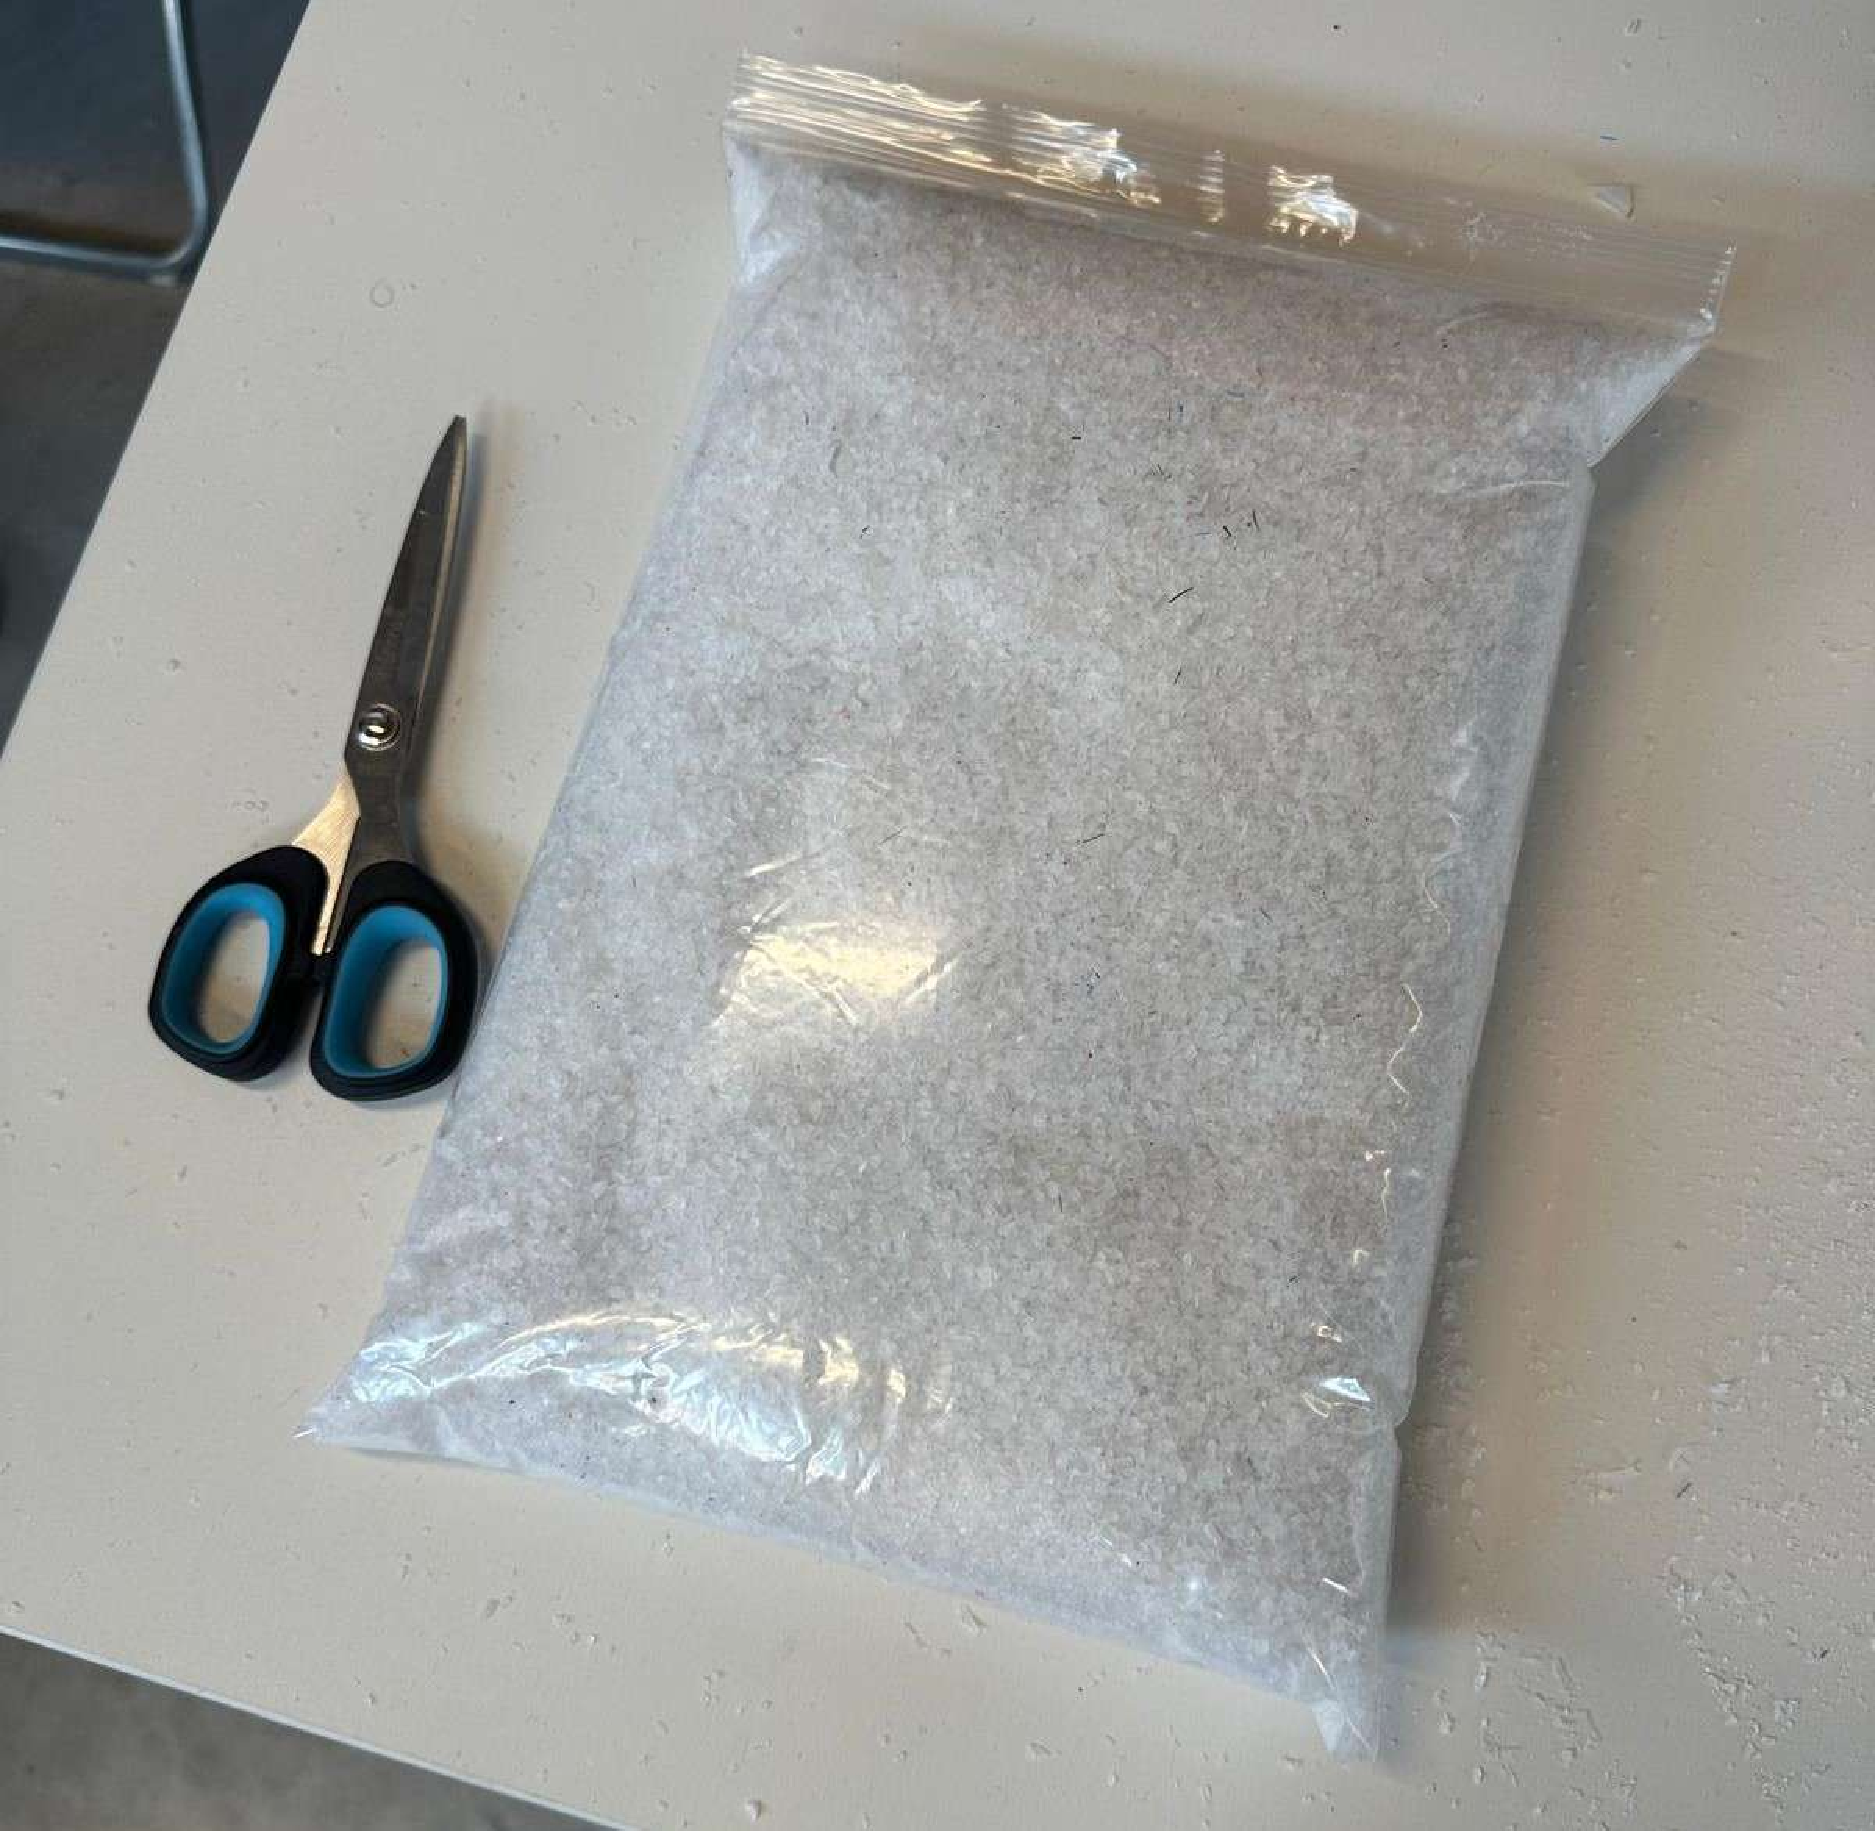
\includegraphics[width = .6\textwidth]{Imagenes/Vectorial/shredded_filament.pdf}
	\caption{Shredded HDPE. Image provided by Gonzalo Alonso García}
	\label{fig:shredded_filament}
\end{figure}

\begin{figure}[h]
	\centering
	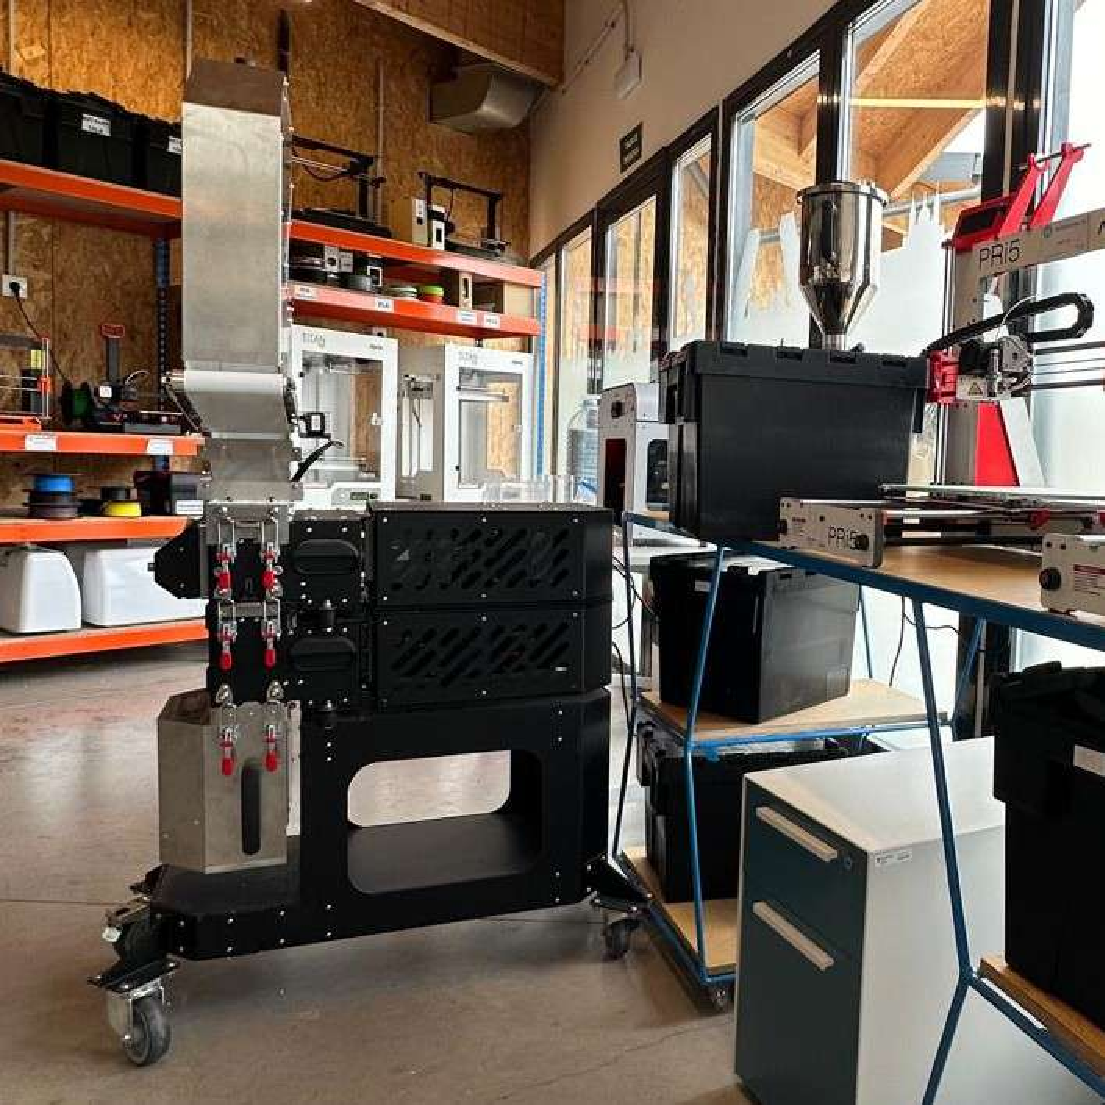
\includegraphics[width = .6\textwidth]{Imagenes/Vectorial/shredder_dryer.pdf}
	\caption{3devo's shredder and dryer. Image provided by Gonzalo Alonso García}
	\label{fig:shredder_dryer}
\end{figure}


\section{Filament Production}
The filament production process was conducted using 3devo's Filament Maker ONE Composer. This 
machine is highly versatile, allowing fine-tuning through the configuration of numerous 
parameters. The most relevant parameters and their impact on filament quality are detailed below.

\subsubsection*{Extrusion and Filament Diameter}
The filamenting machine is equipped with a sensor that continuously measures the diameter of the 
extruded filament. To maintain a consistent diameter, the machine uses a puller mechanism. This 
puller clamps onto the filament and adjusts its speed: increasing the speed when the filament is 
too thick and decreasing it when the filament is too thin. This adjustment process stretches or 
compresses the filament accordingly. Additionally, the machine can produce a graphical 
representation of the filament's diameter over time, aiding in the monitoring and adjustment 
process. This graph can be seen in Figure \ref{fig:filament_graph_2}. It can be seen that the 
diamater is fairly unstable, missing by a considerable margin the targets set by the two 
horizontal lines, delimiting the 1.650 and 1.850 millimeters range.

\begin{figure}[h]
	\centering
	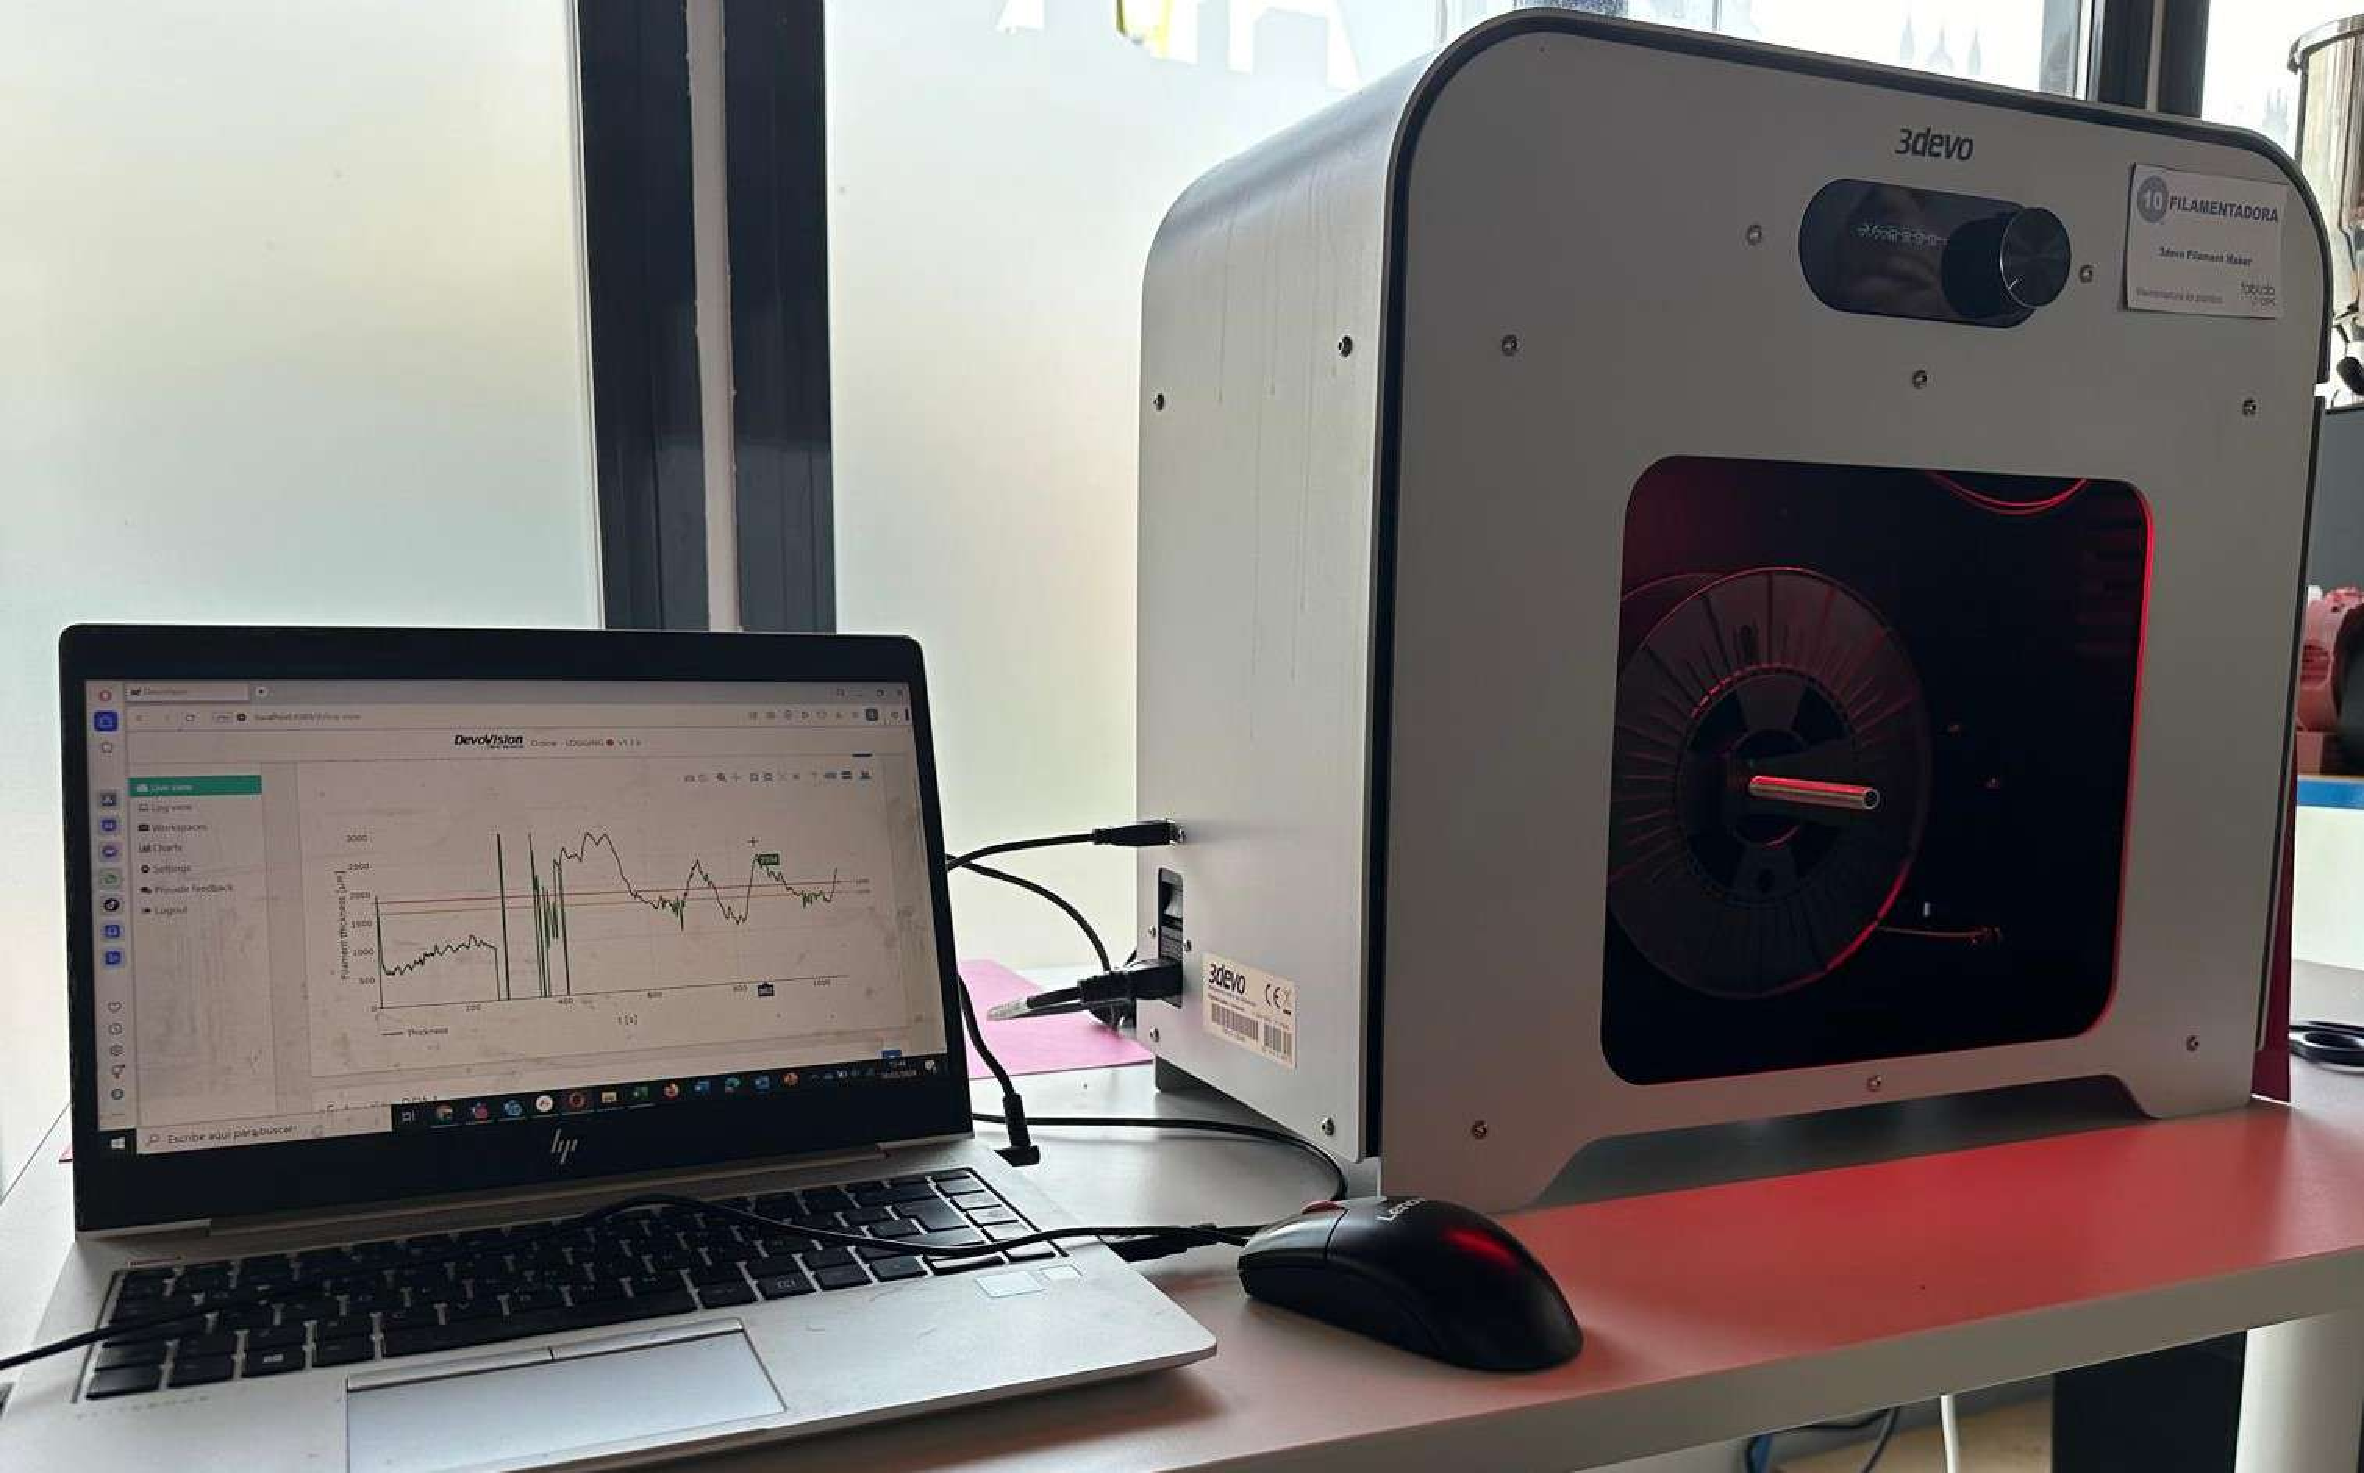
\includegraphics[width = .85\textwidth]{Imagenes/Vectorial/filament_graph_2.pdf}
	\caption{Filament diameter graph with 100\percentsign\ recycled HDPE. Image provided by 
    Gonzalo Alonso García}
	\label{fig:filament_graph_2}
\end{figure}


\subsubsection*{Heaters}
The filamenting machine features four heating zones along an extruder screw that gradually pushes 
the shredded filament through the machine, ultimately extruding it at the end. These heating zones 
are sequentially numbered from 4 to 1, with Zone 4 being the entry point for the shredded plastic 
and Zone 1 being closest to the extruder.

3devo recommends an increasing temperature profile for HDPE, where the temperature is lowest at 
Zone 4 and highest at Zone 1. However, during testing, this setup resulted in an extremely uneven 
filament diameter and a visible texture, indicating incomplete melting and the presence of small 
plastic chunks.

Through extensive experimentation, the team discovered that a decreasing temperature profile 
produced superior results. Starting at approximately 220°C in Zone 4 and reducing the temperature 
to about 170°C in Zone 1 yielded a more consistent and smoother filament. It is speculated that 
this variation in optimal temperature profiles may be due to the recycled nature of the HDPE, 
which alters its melting properties compared to virgin material.

\subsubsection*{Cooling Fans}
Immediately at the extruder's output, two cooling fans are positioned to cool the molten plastic 
as it exits. The speed of these fans needs to be meticulously adjusted to achieve optimal cooling. 
If the plastic is not cooled sufficiently, it remains too soft, causing the puller to crush it. 
Conversely, if the plastic is cooled too much, it becomes too hard, making it difficult for the 
puller to stretch it effectively.

Furthermore, HDPE presents a unique challenge because it consists of two microstructures that 
shrink at different rates when cooled. Rapid cooling can exacerbate this differential shrinkage, 
leading to filament ovalization, a phenomenon where the filament cross-section becomes oval rather 
than circular. This issue is particularly critical because ovalized filament can lead to 
inconsistent extrusion in 3D printers, affecting the quality of the printed parts.

3devo emphasizes the importance of controlled cooling to mitigate these issues\footnote{3devo's 
note on HDPE: \url{https://support.3devo.com/why-is-hdpe-difficult-to-extrude}}. The fans must be 
set to a speed that ensures the plastic is solid enough for handling by the puller but avoids 
rapid cooling that could cause structural inconsistencies. Finding the right balance in fan speed 
is crucial for producing high-quality, round filament that meets the standards required for 
reliable 3D printing. Through careful tuning and testing, the team was able to achieve a cooling 
rate that maintained the filament's integrity and dimensional accuracy.

\section{Challenges and Solutions}

Throughout the filament production process, several challenges emerged. The initial batches of 
extruded filament displayed visible impurities, notably black spots, which resulted in clogging a 
0.4 mm nozzle on the Prusa MK4 3D printer. These impurities are believed to stem from the residual 
dirt on the original plastic containers that were shredded. This underscores the necessity of 
using as-clean-as-possible plastic for shredding to ensure the quality of the final filament.

Another major hurdle was the instability in the filament's diameter. Variations in diameter can 
drastically impact print quality, leading to issues such as under-extrusion when the filament is 
too thin, or even preventing the filament from fitting into the nozzle's 2 mm tube when it is too 
thick. To address this issue, the team experimented with blending virgin HDPE with the shredded 
recycled plastic.

A mixture of 70\percentsign\  recycled HDPE and 30\percentsign\  virgin HDPE yielded significantly 
more stable filament diameter, as illustrated in Figure \ref{fig:filament_graph}. Although a blend 
with 20\percentsign\  virgin HDPE also improved stability, it did not achieve the same level of 
consistency. This blend strategy proved to be a viable solution for mitigating diameter 
instability and improving the overall quality of the filament.

These solutions highlight the importance of both material purity and the strategic use of virgin 
plastic in producing high-quality, reliable 3D printing filament from recycled HDPE. By carefully 
addressing these challenges, the team was able to enhance the performance and usability of the 
recycled filament, paving the way for more sustainable and efficient 3D printing practices.

\begin{figure}[h]
	\centering
	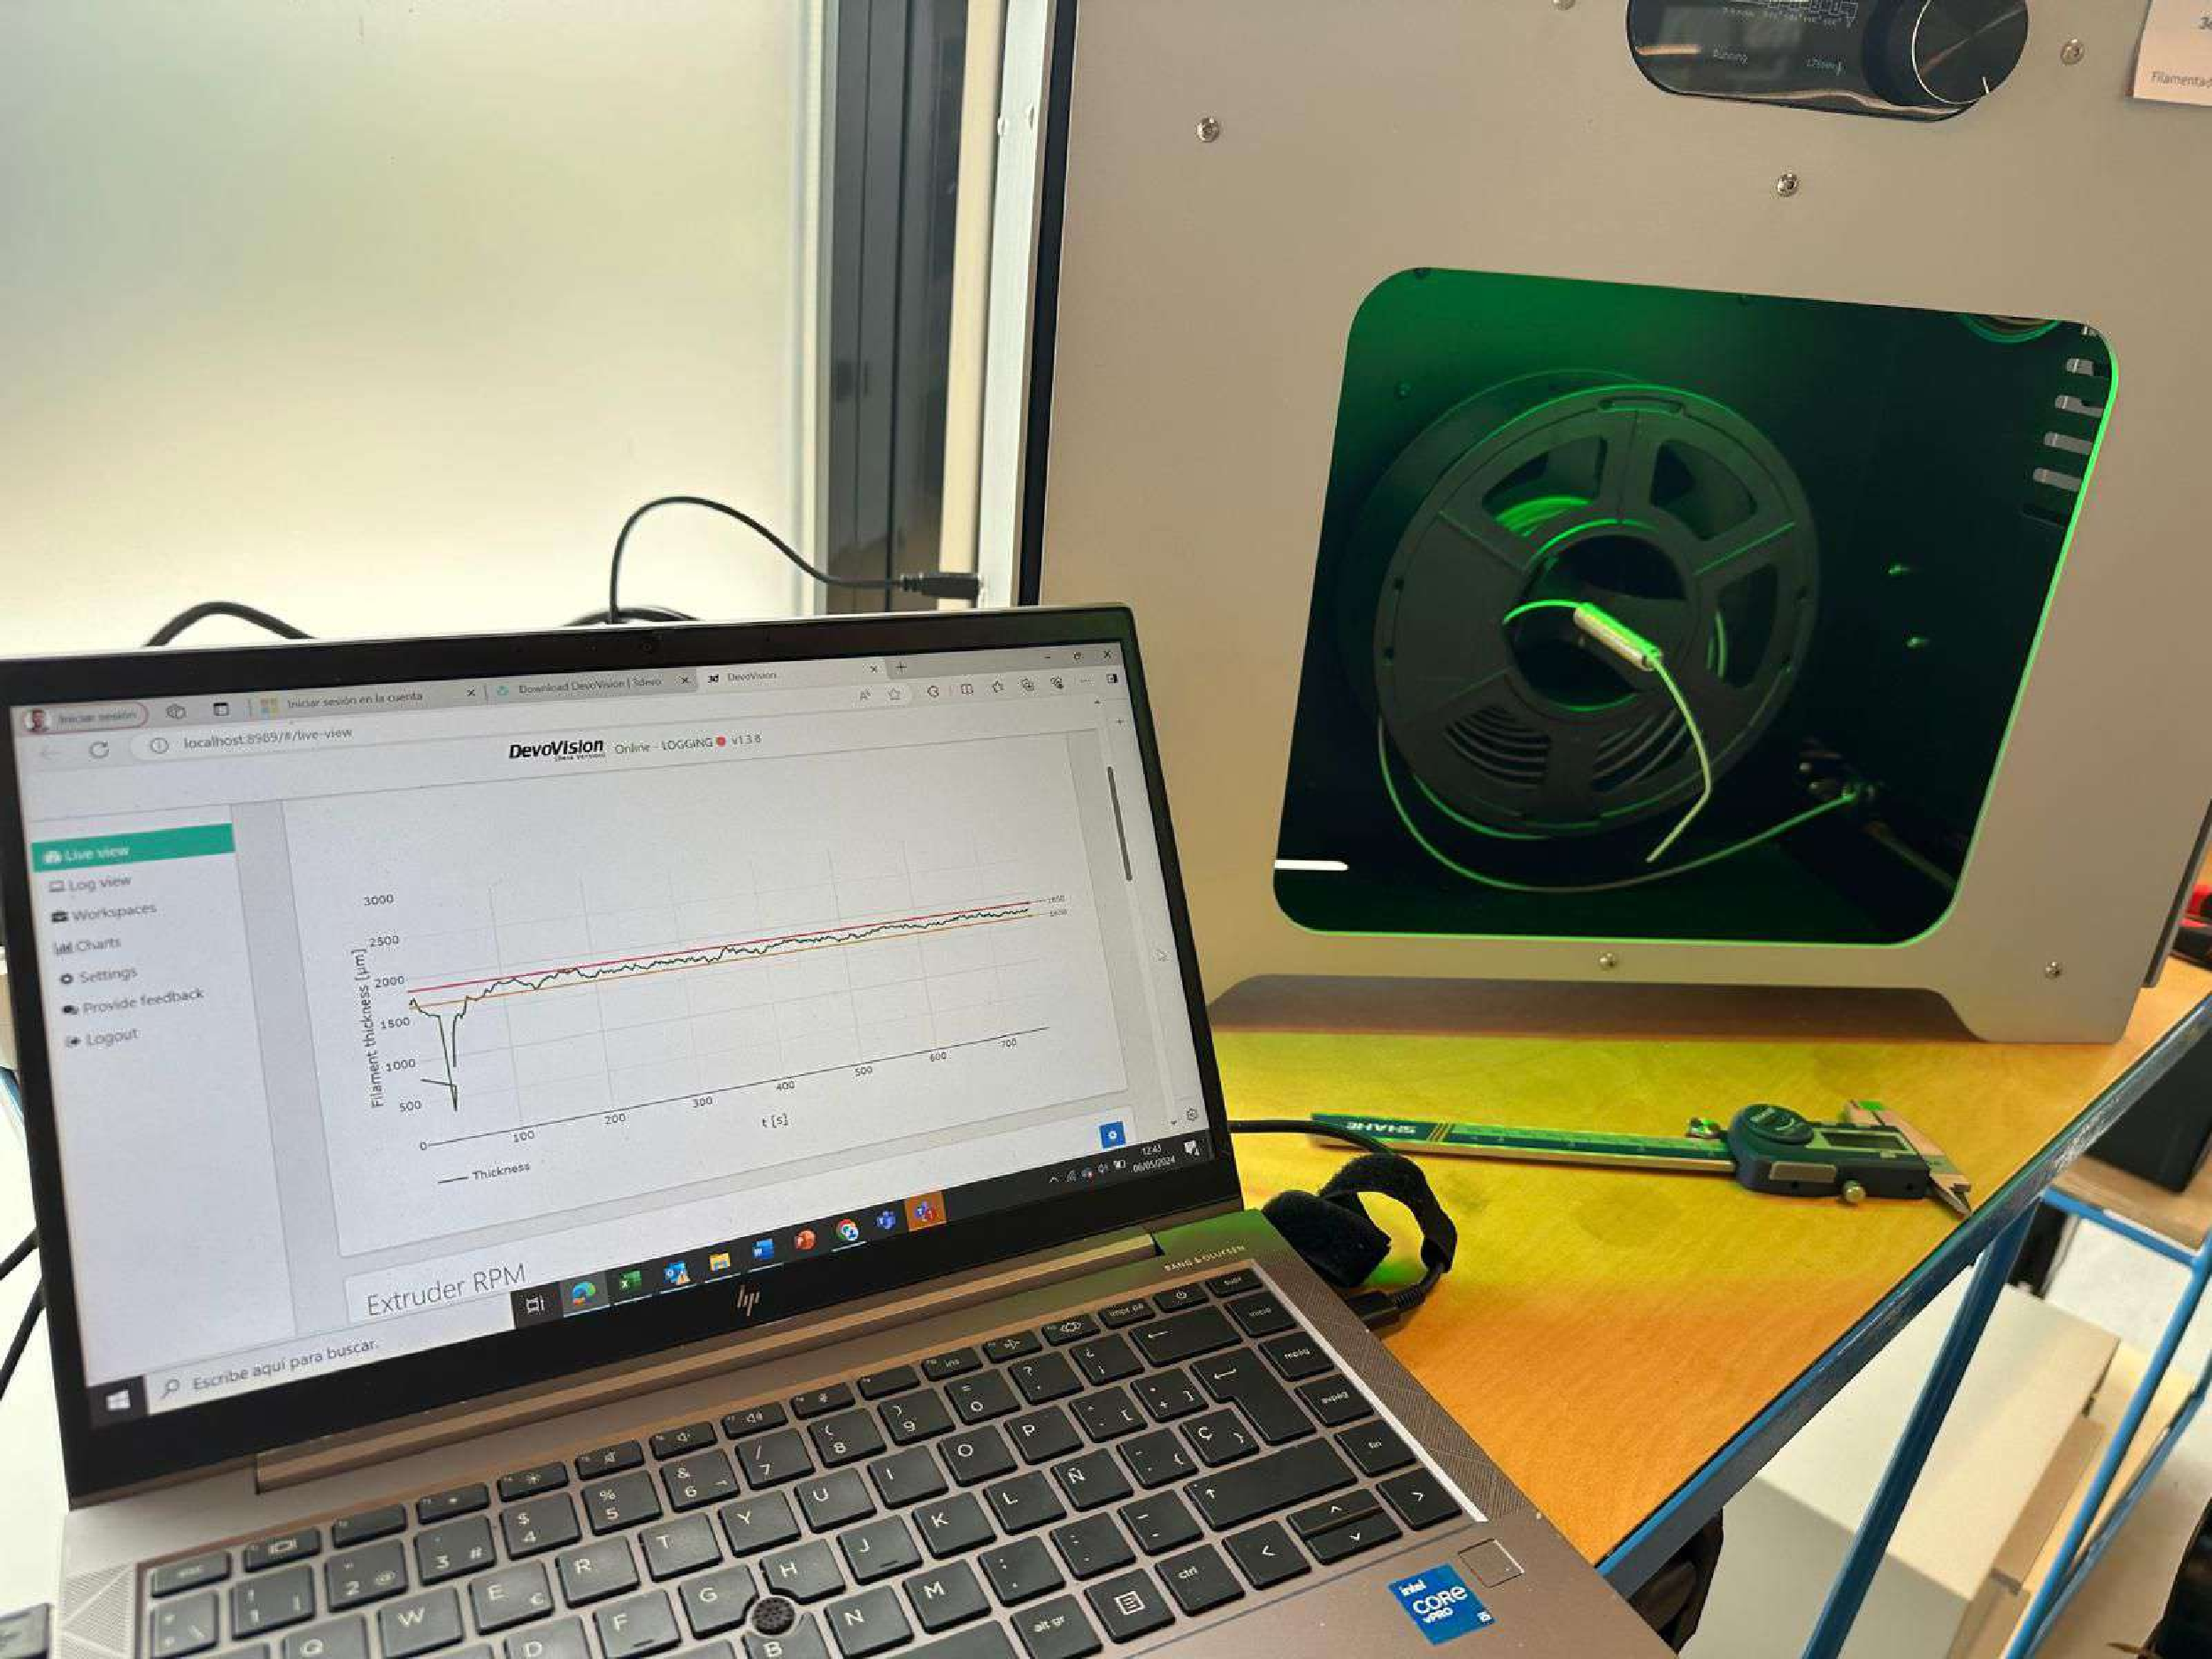
\includegraphics[width = .85\textwidth]{Imagenes/Vectorial/filament_graph.pdf}
	\caption{Filament diameter graph after adding 30\percentsign\ virgin HDPE. Image provided by 
    Gonzalo Alonso García}
	\label{fig:filament_graph}
\end{figure}

\section{Conclusions}
In conclusion, the exploration of recycling HDPE for 3D printing filament has been both 
challenging and enlightening. The initial stages of filament production highlighted critical 
issues such as impurities and diameter instability, both of which were addressed through 
meticulous preparation and the addition of virgin HDPE. These steps ensured a cleaner, more 
consistent filament suitable for 3D printing.

Despite the early setback of a clogged nozzle, the groundwork has been laid for further 
experimentation with 3D printing using this recycled filament. The next phase involves testing the 
printability of HDPE, addressing potential challenges such as warping and adhesion problems that 
are commonly associated with this material. With the setup now optimized, future trials will focus 
on overcoming these obstacles to fully realize the potential of recycled HDPE in 3D printing 
applications.

The collaboration with the Sustainability team and the support from the ``Centro de Innovación en 
Economía Circular'' have been invaluable, demonstrating the feasibility and benefits of 
integrating circular economy principles into technological projects.

% \chapter{Título del Apéndice B}
\label{Appendix:Key2}

Se pueden añadir los apéndices que se consideren oportunos.
%\include{Apendices/appendixC}
%\include{...}
%\include{...}
%\include{...}
\backmatter



%
% Índice de palabras
%

% Sólo  la   generamos  si  está   declarada  \generaindice.  Consulta
% TeXiS.sty para más información.

% En realidad, el soporte para la generación de índices de palabras
% en TeXiS no está documentada en el manual, porque no ha sido usada
% "en producción". Por tanto, el fichero que genera el índice
% *no* se incluye aquí (está comentado). Consulta la documentación
% en TeXiS_pream.tex para más información.
\ifx\generaindice\undefined
\else
%%---------------------------------------------------------------------
%
%                        TeXiS_indice.tex
%
%---------------------------------------------------------------------
%
% TeXiS_indice.tex
% Copyright 2009 Marco Antonio Gomez-Martin, Pedro Pablo Gomez-Martin
%
% This file belongs to TeXiS, a LaTeX template for writting
% Thesis and other documents. The complete last TeXiS package can
% be obtained from http://gaia.fdi.ucm.es/projects/texis/
%
% This work may be distributed and/or modified under the
% conditions of the LaTeX Project Public License, either version 1.3
% of this license or (at your option) any later version.
% The latest version of this license is in
%   http://www.latex-project.org/lppl.txt
% and version 1.3 or later is part of all distributions of LaTeX
% version 2005/12/01 or later.
%
% This work has the LPPL maintenance status `maintained'.
% 
% The Current Maintainers of this work are Marco Antonio Gomez-Martin
% and Pedro Pablo Gomez-Martin
%
%---------------------------------------------------------------------
%
% Contiene  los  comandos  para  generar  el índice  de  palabras  del
% documento.
%
%---------------------------------------------------------------------
%
% NOTA IMPORTANTE: el  soporte en TeXiS para el  índice de palabras es
% embrionario, y  de hecho  ni siquiera se  describe en el  manual. Se
% proporciona  una infraestructura  básica (sin  terminar)  para ello,
% pero  no ha  sido usada  "en producción".  De hecho,  a pesar  de la
% existencia de  este fichero, *no* se incluye  en Tesis.tex. Consulta
% la documentación en TeXiS_pream.tex para más información.
%
%---------------------------------------------------------------------


% Si se  va a generar  la tabla de  contenidos (el índice  habitual) y
% también vamos a  generar el índice de palabras  (ambas decisiones se
% toman en  función de  la definición  o no de  un par  de constantes,
% puedes consultar modo.tex para más información), entonces metemos en
% la tabla de contenidos una  entrada para marcar la página donde está
% el índice de palabras.

\ifx\generatoc\undefined
\else
   \addcontentsline{toc}{chapter}{\indexname}
\fi


% Generamos el índice
\printindex

% Variable local para emacs, para  que encuentre el fichero maestro de
% compilación y funcionen mejor algunas teclas rápidas de AucTeX

%%%
%%% Local Variables:
%%% mode: latex
%%% TeX-master: "./tesis.tex"
%%% End:

\fi

%
% Lista de acrónimos
%

% Sólo  lo  generamos  si  está declarada  \generaacronimos.  Consulta
% TeXiS.sty para más información.


\ifx\generaacronimos\undefined
\else
%---------------------------------------------------------------------
%
%                        TeXiS_acron.tex
%
%---------------------------------------------------------------------
%
% TeXiS_acron.tex
% Copyright 2009 Marco Antonio Gomez-Martin, Pedro Pablo Gomez-Martin
%
% This file belongs to TeXiS, a LaTeX template for writting
% Thesis and other documents. The complete last TeXiS package can
% be obtained from http://gaia.fdi.ucm.es/projects/texis/
%
% This work may be distributed and/or modified under the
% conditions of the LaTeX Project Public License, either version 1.3
% of this license or (at your option) any later version.
% The latest version of this license is in
%   http://www.latex-project.org/lppl.txt
% and version 1.3 or later is part of all distributions of LaTeX
% version 2005/12/01 or later.
%
% This work has the LPPL maintenance status `maintained'.
% 
% The Current Maintainers of this work are Marco Antonio Gomez-Martin
% and Pedro Pablo Gomez-Martin
%
%---------------------------------------------------------------------
%
% Contiene  los  comandos  para  generar  el listado de acrónimos
% documento.
%
%---------------------------------------------------------------------
%
% NOTA IMPORTANTE:  para que la  generación de acrónimos  funcione, al
% menos  debe  existir  un  acrónimo   en  el  documento.  Si  no,  la
% compilación  del   fichero  LaTeX  falla  con   un  error  "extraño"
% (indicando  que  quizá  falte  un \item).   Consulta  el  comentario
% referente al paquete glosstex en TeXiS_pream.tex.
%
%---------------------------------------------------------------------


% Redefinimos a español  el título de la lista  de acrónimos (Babel no
% lo hace por nosotros esta vez)

\def\listacronymname{Lista de acrónimos}

% Para el glosario:
% \def\glosarryname{Glosario}

% Si se  va a generar  la tabla de  contenidos (el índice  habitual) y
% también vamos a  generar la lista de acrónimos  (ambas decisiones se
% toman en  función de  la definición  o no de  un par  de constantes,
% puedes consultar config.tex  para más información), entonces metemos
% en la  tabla de contenidos una  entrada para marcar  la página donde
% está el índice de palabras.

\ifx\generatoc\undefined
\else
   \addcontentsline{toc}{chapter}{\listacronymname}
\fi


% Generamos la lista de acrónimos (en realidad el índice asociado a la
% lista "acr" de GlossTeX)

\printglosstex(acr)

% Variable local para emacs, para  que encuentre el fichero maestro de
% compilación y funcionen mejor algunas teclas rápidas de AucTeX

%%%
%%% Local Variables:
%%% mode: latex
%%% TeX-master: "../Tesis.tex"
%%% End:

\fi

%
% Final
%
% %---------------------------------------------------------------------
%
%                      fin.tex
%
%---------------------------------------------------------------------
%
% fin.tex
% Copyright 2009 Marco Antonio Gomez-Martin, Pedro Pablo Gomez-Martin
%
% This file belongs to the TeXiS manual, a LaTeX template for writting
% Thesis and other documents. The complete last TeXiS package can
% be obtained from http://gaia.fdi.ucm.es/projects/texis/
%
% Although the TeXiS template itself is distributed under the 
% conditions of the LaTeX Project Public License
% (http://www.latex-project.org/lppl.txt), the manual content
% uses the CC-BY-SA license that stays that you are free:
%
%    - to share & to copy, distribute and transmit the work
%    - to remix and to adapt the work
%
% under the following conditions:
%
%    - Attribution: you must attribute the work in the manner
%      specified by the author or licensor (but not in any way that
%      suggests that they endorse you or your use of the work).
%    - Share Alike: if you alter, transform, or build upon this
%      work, you may distribute the resulting work only under the
%      same, similar or a compatible license.
%
% The complete license is available in
% http://creativecommons.org/licenses/by-sa/3.0/legalcode
%
%---------------------------------------------------------------------
%
% Contiene la última página
%
%---------------------------------------------------------------------


% Ponemos el marcador en el PDF
\ifpdf
   \pdfbookmark{Fin}{fin}
\fi

\thispagestyle{empty}\mbox{}

Este texto se puede encontrar en el fichero Cascaras/fin.tex. Si deseas eliminarlo, basta con comentar la línea correspondiente al final del fichero TFGTeXiS.tex.

\vspace*{4cm}

\small

\hfill \emph{--¿Qué te parece desto, Sancho? -- Dijo Don Quijote --}

\hfill \emph{Bien podrán los encantadores quitarme la ventura,}

\hfill \emph{pero el esfuerzo y el ánimo, será imposible.}

\hfill 

\hfill \emph{Segunda parte del Ingenioso Caballero} 

\hfill \emph{Don Quijote de la Mancha}

\hfill \emph{Miguel de Cervantes}

\vfill%space*{4cm}

\hfill \emph{--Buena está -- dijo Sancho --; fírmela vuestra merced.}

\hfill \emph{--No es menester firmarla -- dijo Don Quijote--,}

\hfill \emph{sino solamente poner mi rúbrica.}

\hfill 

\hfill \emph{Primera parte del Ingenioso Caballero} 

\hfill \emph{Don Quijote de la Mancha}

\hfill \emph{Miguel de Cervantes}


\newpage
\thispagestyle{empty}\mbox{}

\newpage

% Variable local para emacs, para  que encuentre el fichero maestro de
% compilación y funcionen mejor algunas teclas rápidas de AucTeX

%%%
%%% Local Variables:
%%% mode: latex
%%% TeX-master: "../Tesis.tex"
%%% End:

\end{otherlanguage}
\end{document}
